\chapter{Results}
\label{ch:results}
	\section{Proximate deforestation drivers}
	\label{sec:results_deforestation}

		\subsection{Forest definition}
		\label{subsec:results_forest_definition}
			Our goal is to determine at which canopy cover density the agreement between \ac{GL30} and \ac{GFC} tree cover is greatest to obtain the subsequent \ac{PDD} for stable \ac{LC} transitions introduced by anthropogenic causes. This process should ensure that we keep the largest number of tree cover loss samples from the \ac{GFC} dataset while harmonizing the tree cover definition between both layers. Our initial hypothesis was that the tree cover agreement is at its maximum within the canopy density interval of $(30,100]$ for the entire study extent. We assumed that for Latin America and Asia/Australia the best results could be achieved with the same canopy density threshold. For Africa we assumed that the highest agreement could be achieved within the interval of $(10,100]$ because this region comprises a higher frequency of sparse woodland cover. The following paragraphs present our results for the three regions in the following order: Latin America, Asia/Australia and Africa. The last paragraph discusses the results for the entire study extent and determines which canopy density we used for the following \ac{PDD} prediction.
			\begin{figure}[ht]
				\centering
				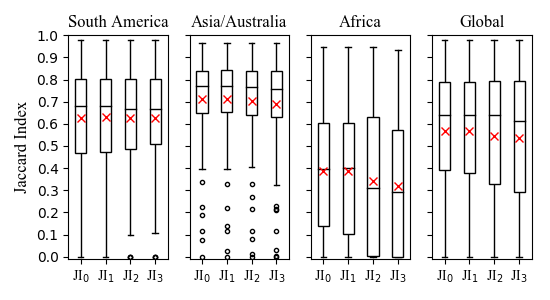
\includegraphics[scale=.91]{img/jaccard}
				\caption[Tree cover similarity distribution]{\textbf{Tree cover similarity distribution:} This box-plot shows the distribution of Jaccard Indexes for each raster image tile pair of GlobeLand30 and Global Forest Change tree cover from 2000. The labels $JI_0$, $JI_1$, $JI_2$, and $JI_3$ on the x-axis account for the canopy density classes $(0,100]$, $(10,100]$, $(20,100]$, and $(30,100]$, respectively. The y-axis is the Jaccard Index of the corresponding raster image pair, where 0 is a total disagreement and 1 a total agreement. Red crosses within the $Q_{25}$, $Q_{50}$, and $Q_{75}$ boxes highlight the sample mean. Whiskers are 1.5 times the $IQR$.}
				\label{fig:jaccard}
			\end{figure}

			For Latin America figure \ref{fig:jaccard} shows the distribution of the computed \acp{JI} for all tile pairs within the canopy density intervals. The sample mean does not change significantly within the four canopy density experiments. It is approximately 0.62 while sample median decreases from 0.68 to 0.66 from the interval class to the last. The upper 25 \% of the first experiment interval have a tree cover similarity ranging between approximately 0.8 and 1. This holds true over the other three experiments while only the maximum similarity slightly increases from 0.9787 to 0.9798. The figure \ref{fig:jaccard_americas_appendix} in the appendix \ref{ch:appendix_b} suggests, that exclusions of canopy densities smaller than 11\% increases slightly the tree cover agreement of the upper 25\% but the exclusion of higher canopy density provides no benefit. This can be explained by the fact that the upper percentile already contain samples with a high tree cover agreement and it is to assume that only a small number of pixels have canopy density smaller than 30. Therefore, the interval change has only a small impact on this samples. For the first two canopy density intervals the range of the lower 25\% percentile is between approximately 0.0003 and 0.45. Whereas the range increases from 0.0 to 0.5 for the last two interval classes. The figure \ref{fig:jaccard_americas_appendix} reveals a strong regional dependency of tree cover agreement within different canopy density classes of the lower percentiles. Whereas samples from the northern hemisphere show a decline in agreement the samples of the southern hemisphere show a increase of agreement. The strong up-shift of the southern samples within the last two intervals increases the range of lower percentile. This suggests in general that samples with low tree cover agreement benefit by the exclusion of lower canopy densities. The mobility of the samples within the $Q_1$ and $Q_3$ percentile show no general trend. For the first two experiments it ranges between 0.5 and 0.8 and for the last two it shows a small decline in $IQR$. This suggests that tiles within this group could benefit from a local optimization of canopy density exclusion. We applied a Wilcoxon signed-rank test to deduce which canopy density class yields the highest tree cover agreement overall samples in Latin America. Table \ref{tab:wilcoxontwosided_regions} shows the results for the two-sided test and table \ref{tab:wilcoxontwosided_regions} for the one-sided test. The two-sided test reveals that only the similarity distribution between $JI_0$ and $JI_1$ is significantly different ($p<0.01$), while the comparison of the other distributions suggest that they are equal. The directional test of $JI_0$ and $JI_1$ suggests that the regional tree cover agreement is significantly greater ($p<0.005$) if canopy densities smaller than 10 are excluded. The directional test does not confirm that the distribution if $JI_1$ is significantly greater than $JI_2$ and $JI_3$. Therefore it can be assumed that the exclusion of lower canopy densities could yield better results for certain tiles. The result of our experiments suggests that the tree cover agreement between \ac{GL30} and \ac{GFC} at canopy densities greater than 10 is at its maximum for Latin America. In case of local studies or for smaller extents the canopy density should be selected by a single tile approach to optimize the tree cover agreement by maximizing the number of data points of the \ac{GFC} dataset.
			\begin{table}[ht]
				\centering
				\caption[Continental experiment group comparison]{\textbf{Continental experiment group comparison:} This table shows the results of a two-sided Wilcoxon signed-rank test to detect continental differences in the tree cover agreement by considering different canopy densities between GlobeLand30 and Global Forest Change at 2000. The classes $JI_0$, $JI_1$, $JI_2$, and $JI_3$ as row and column headings account for the canopy density classes (0,100], (10,100], (20,100], and (30,100], respectively. The test hypothesis is H$_0$: $X_1=X_2$ where $X_1$ is the column $JI_n$ class and $X_2$ the row $JI_n$ class. The significance is indicated by $p^{*}<0.05$, $p^{**}<0.02$, and $p^{***}<0.01$.}
				\label{tab:wilcoxontwosided_regions}
				\begin{tabular}{llllllllllll}
					\hline
					& \multicolumn{3}{c}{Latin America} && \multicolumn{3}{c}{Asia/Australia} && \multicolumn{3}{c}{Africa} \\\cline{2-4}\cline{6-8}\cline{10-12}
					Cls & JI$_0$ & JI$_1$ & JI$_2$ && JI$_0$ & JI$_1$ & JI$_2$ && JI$_0$ & JI$_1$ & JI$_2$ \\\hline
					JI$_1$ & .00$^{***}$ & - & - && .71 & - & - && .22 & - & - \\
					JI$_2$ & .30 & 1. & - && .00$^{***}$ & .00$^{***}$ & - && .09 & .09  & - \\
					JI$_3$ & .64 & 1. & 1. && .00$^{***}$ & .00$^{***}$ & .00$^{***}$ && .00$^{***}$ & .00$^{***}$ & .00$^{***}$ \\\hline
				\end{tabular}
			\end{table}
			\begin{table}[ht]
				\centering
				\caption[Continental experiment group directional comparison]{\textbf{Continental experiment group directional comparison:} This table shows the results of a one-sided Wilcoxon signed-rank test to detect the direction of continental differences in the tree cover agreement by considering different canopy densities between GlobeLand30 and Global Forest Change at 2000. The classes $JI_0$, $JI_1$, $JI_2$, and $JI_3$ as row and column headings account for the canopy density classes (0,100], (10,100], (20,100], and (30,100], respectively. The test hypothesis is H$_0$: $X_1\leq X_2$ and H$_0$: $X_2\geq X_1$ where $X_1$ is the column $JI_n$ class and $X_2$ the row $JI_n$ class. The significance is indicated by $p^{*}<0.05$, $p^{**}<0.025$, $p^{***}<0.01$, and $p^{\dagger}<0.005$.}
				\label{tab:wilcoxononesided_regions}
				\begin{tabular}{lllllllllllllll}
					\hline
					& \multicolumn{4}{c}{Latin America} && \multicolumn{4}{c}{Asia/Australia} && \multicolumn{4}{c}{Africa} \\\cline{2-5}\cline{7-10}\cline{12-15}
					Cls & JI$_0$ & JI$_1$ & JI$_2$ & JI$_3$ && JI$_0$ & JI$_1$ & JI$_2$ & JI$_3$ && JI$_0$ & JI$_1$ & JI$_2$ & JI$_3$ \\\hline
					JI$_0$ & - & .00$^{\dagger}$ & .14 & .33 && - & 1. & 1. & 1. && - & .65 & 1. & 1. \\
					JI$_1$ & 1. & - & .55 & .55 && .36 & - & 1. & 1. && .89 & - & 1. & 1. \\
					JI$_2$ & 1. & 1. & - & .55 && .00$^{\dagger}$ & .00$^{\dagger}$ & - & 1. && .03$^{*}$ & .03$^{*}$ & - & 1. \\
					JI$_3$ & 1. & 1. & 1. & - && .00$^{\dagger}$ & .00$^{\dagger}$ & .00$^{\dagger}$ & - && .00$^{\dagger}$ & .00$^{\dagger}$ & .00$^{\dagger}$ & - \\\hline
				\end{tabular}
			\end{table}

			For Asia/Australia, the sample mean scatters around 0.7 as the red crosses in figure \ref{fig:jaccard} suggest. The sample mean decreases slightly at higher canopy density intervals. Further, the median is approximately 0.8 by showing a slight decrease at higher canopy density intervals too. The range of the upper percentiles for all experiments groups is between approximately 0.85 and 0.96 while the maximum agreement decreases slightly from 0.9654 to 0.9634. Figure \ref{fig:jaccard_asia_appendix} in the appendix \ref{ch:appendix_b}, reveals that in general the tree cover agreement increases if canopy densities below 10 \% are excluded but the exclusion of densities above 20 \% reverts this. For Asia/Australia the lower percentile ranges between approximately 0 and 0.65 while most of the samples show a decline in tree cover agreement if canopy densities above 20 are excluded. Within the $Q_1,3$ percentile a per tile relationship is detectable. The range of this percentile is between 0.65 and 0.85 for the first two classes $JI_0$ and $JI_1$ while the range increases for the last two experiments. As mentioned no clear trend is observable some of the samples benefit if the considered canopy density interval is increased till 30 \% and some show a decrease in agreement if the canopy density is lift over 10 \%. The two-sided Wilcoxon test in table \ref{tab:wilcoxontwosided_regions} reveals that the similarity distribution is significantly different (p<0.01) between each experiment group except the pair of $JI_1$ and $JI_0$. The directional test in table \ref{tab:wilcoxononesided_regions} reveals that the tree cover agreement distributions of $JI_2$ and $JI_3$ are significantly smaller than $JI_0$ and $JI_1$ (p<0.005). Further this results show that the distributions of $JI_0$ and $JI_1$ have no directional differences. This could be explained by a regional or tile-wise agreement component. While some of the tiles show strong increase in similarity if canopy density is set to 10 \%, others show a decrease. A more detailed analysis could be performed by applying a smaller canopy density step-size. For studies targeting the region Asia/Australia the results of the directional tests suggest to use all data from \ac{GFC} within the canopy density interval of $(0,100]$. While the figure \ref{fig:jaccard_asia_appendix} suggests to include all data form the interval $(10,100]$.

			The box-plot for Africa in figure \ref{fig:jaccard} shows that the similarity range of the upper 75 \% is the greatest among our study regions. It ranges between 0.15 and 1.0 for $JI_0$ while the range increases if smaller canopy densities are excluded. The first two experiment groups $JI_0$ and $JI_1$ have a nearly similar mean and median of approximately 0.38 and 0.4, respectively. Whereas both metrics show a strong decline to 0.33 and 0.3 in the last two experiment groups $JI_2$ and $JI_3$, respectively. Figure \ref{fig:jaccard_africa_appendix} in the appendix \ref{ch:appendix_b} reveals that the upper 25 \% different to Latin America and Asia not benefit in general by exclusion of lower canopy densities. Africa has the highest amount of tiles where there tree cover agreement is smaller than 0.1. For the second experiment group $JI_1$ 11 tiles from the \ac{AISM} have a complete disagreement ($JI=0$) if the canopy density interval is reduced to $(10,100]$. This trend continues if the canopy density interval is further reduced. This already suggests that reducing the canopy density interval for Africa is not feasible. The two-sided test in table \ref{tab:wilcoxontwosided_regions} reveals that $JI_3$ is significantly different ($p<0.01$) in its similarity distribution compared to the other experiment groups $JI_0$, $JI_1$, and $JI_2$, respectively. The other experiment groups could origin from the same similarity distribution. Especially, the tree cover agreement between $JI_0$ and $JI_1$ show evidences that it could origin from the same distribution. This is comparable with the Asia/Australian region. The table \ref{tab:wilcoxononesided_regions} shows the directional component of the tree cover agreement between the experiments groups for Africa. The tree cover agreement of $JI_2$ and $JI_3$ is significantly smaller than $JI_0$ or $JI_1$ as the table suggest. Therefore the exclusion of canopy densities above 10 \% reduces the continental tree cover agreement in Africa. For the two experiment groups $JI_0$ and $JI_1$ no directional agreement component could be proofed but the figure \ref{fig:jaccard_africa_appendix} shows a strong regional component of tree cover agreement. The strong regional component can be explained by the high share of sparse woodland in Africa. The figure \ref{fig:africa_tree_cover} in section \ref{subsec:results_tree_cover_and_deforestation} shows that different from Asia/Australia and Latin America a vast amount of African tree cover has a canopy density between 0 and 46 \%. The results for Africa suggests to set the canopy density interval to $(0,100]$ to optimize the tree cover agreement between \ac{GL30} and \ac{GFC} on a continental level. Preferable the strong regional component suggests to optimize the tree cover agreement per tile to achieve a higher tree cover agreement for the entire continent.

			The table \ref{tab:wilcoxononesided_comparison} in the appendix \ref{ch:appendix_b} shows that in Asia/Australia the tree cover similarity between \ac{GL30} and \ac{GFC} is the greatest out of all three regions. Only within the last experiment group $JI_3$ the median tree cover agreement between Asia/Australia and Latin America could be the same shown in table \ref{tab:wilcoxontwosided_comparison}. Africa has the poorest tree cover agreement out of our three continental regions. Asia's higher tree cover agreement compared to Latin America could relate to the smaller total landmass and vice versa forest cover within this region and the high share of dense forest cover. Therefore both global \ac{LC} datasets have a smaller chance to miss forest covered pixels. That both regions achieve better tree cover similarity as Africa could be explained by the high amount of dense forest cover within this regions. It could be assumed that the probability of misclassification of forest cover increases as lower the canopy density is. In regards of tile-wise tree cover agreement optimization would Africa benefit at most out of the three regions. In Asia/Australia and Latin America only certain tiles would benefit from a exclusive optimization as the figures \ref{fig:jaccard_americas_appendix} and \ref{fig:jaccard_asia_appendix} suggests.

			On the far right of figure \ref{fig:jaccard} the tree cover agreement of the entire study extent is shown. The sample mean and median differ between the first two experiment groups and the last two groups. For the first two groups the mean and median account for 0.56 and 0.63, respectively. The last two experiment groups show a decline to 0.53 and 0.53 for mean and median. For the upper percentile the same statement as for the regions holds true. In general, the samples with high tree cover agreement benefit from the exclusion of lower canopy densities. The lower percentile shows strong regional or tile-wise tree agreement dependencies. If we consider the entire sample range the mid percentile steadily increases its range from 0.4 to 0.8 till 0.3 to 0.8. As mentioned in the regional analysis, this percentile is characterized by inhomogeneous changes of tree cover agreement by the step-wise change of the canopy density. In general the trend points downwards as the decrease in median and the range increase show. The results of the two-sided Wilcoxon test in table \ref{tab:wilcoxontwosided_all} show a significant difference in distribution (p<0.02 and p<0.01) between each experiment group except $JI_0$ and $JI_2$ where the similarity distribution could be the same. Table \ref{tab:wilcoxononesided_all} highlights the directional component of these distribution differences. At a global scale the tree cover agreement is at its maximum if we set the canopy density interval to $(10,100]$. The second experiment group $JI_1$ is significantly greater than $JI_0$ (p<0.005) and the last two groups $JI_2$ and $JI_3$ are significantly smaller (p>0.005) than $JI_1$. Further, the tree cover agreement of $JI_0$ is significantly greater than (p<0.005 and p<0.05) $JI_2$ and $JI_3$. Therefore it is proved that canopy densities above 20 \% reduce the tree cover agreement between \ac{GL30} and \ac{GFC} on a global level. On a global scale as the analysis on tree cover agreement suggests the highest agreement can be achieved within the $JI_1$ interval. Therefore we decided to proceed for our study of \ac{PDD} and the derived products with this definition of tree cover.
			\begin{table}[ht]
				\centering
				\caption[Global experiment group comparison]{\textbf{Global experiment group comparison:} This table shows a two-sided Wilcoxon signed-rank test to detect differences in the tree cover agreement by considering different canopy densities between GlobeLand30 and Global Forest Change at 2000. The classes $JI_0$, $JI_1$, $JI_2$, and $JI_3$ as row and column headings account for the canopy density classes (0,100], (10,100], (20,100], and (30,100], respectively. The test hypothesis is H$_0$: $X_1=X_2$ where $X_1$ is the column $JI_n$ class and $X_2$ the row $JI_n$ class. The significance is indicated by $p^{*}<0.05$, $p^{**}<0.02$, and $p^{***}<0.01$.}
				\label{tab:wilcoxontwosided_all}
				\begin{tabular}{llll}
					\hline
					Cls & JI$_0$ & JI$_1$ & JI$_2$ \\\hline
					JI$_1$ & .01$^{**}$ & - & - \\
					JI$_2$ & .07 & .04$^{*}$ & - \\
					JI$_3$ & .00$^{***}$ & .00$^{***}$ & .00$^{***}$ \\\hline
				\end{tabular}
			\end{table}
			\begin{table}[ht]
				\centering
				\caption[Global experiment group directional comparison]{\textbf{Global experiment group directional comparison:} This table shows a one-sided Wilcoxon test to determine the direction of global differences in the tree cover agreement by considering different canopy densities between GlobeLand30 and Global Forest Change at 2000. The test hypothesis is H$_0$: $X_1\leq X_2$ and H$_0$: $X_2\geq X_1$ where $X_1$ is the column $JI_n$ class and $X_2$ the row $JI_n$ class. The significance is indicated by $p^{*}<0.05$, $p^{**}<0.025$, $p^{***}<0.01$, and $p^{\dagger}<0.005$.}
				\label{tab:wilcoxononesided_all}
				\begin{tabular}{lllll}
					\hline
					Cls & JI$_0$ & JI$_1$ & JI$_2$ & JI$_3$ \\\hline
					JI$_0$ & - & .01$^{***}$ & 1. & 1. \\
					JI$_1$ & 1. & - & 1. & 1. \\
					JI$_2$ & .07 & .03$^{*}$ & - & 1. \\
					JI$_3$ & .00$^{\dagger}$ & .00$^{\dagger}$ & .00$^{\dagger}$ & - \\\hline
				\end{tabular}
			\end{table}

		%old text
		%For Latin America, Asia/Australia and Africa as well the entire study extent figure \ref{fig:jaccard} shows the distribution of the computed \acp{JI} for all tile pairs within the canopy density intervals. The x-axis are the different canopy density intervals where the label $JI_0$ accounts for $(0,100]$, $JI_1$ $(10,100]$, $JI_2$ $(20,100]$, and $JI_3$ $(30,100]$, respectively. The y-axis is the corresponding \ac{JI} between 0 and 1 where 0 highlights a complete disagreement and 1 a full agreement. The sample mean is labelled by a red cross and the boxes comprises the $Q_1$ (25 \%), $Q_2$ (50 \%), and $Q_3$ (75 \%) sample interval, respectively.

		%old intro
		%Our goal is to determine at which canopy cover density the agreement between \ac{GL30} and \ac{GFC} tree cover is greatest to receive the subsequent \ac{PDD} for stable \ac{LC} transitions introduced by anthropogenic causes. This process should ensure that we keep the largest number of tree cover loss samples from the \ac{GFC} dataset while harmonizing the tree cover definition between both layers. We applied the \ac{JI} to determine the similarity between each tile pair from our \ac{AISM}. The \ac{JI} computation is grouped by the continental regions Latin America (82 tiles), Asia/Australia (86 tiles), and Africa (101 tiles). We determined the similarity for the following canopy density intervals: $(0, 100]$, $(10, 100]$, $(20, 100]$, and $(30, 100]$. Later we excluded all tiles with a initial \ac{JI} (canopy density interval $(0,100]$) from our analysis because these tile pair does not contain any tree cover. We excluded 6, 9, and 15 tiles for Latin America, Asia/Australia and Africa, respectively. To determine the canopy density interval where the agreement is at maximum we applied the non-parametric tests Wilcoxon signed-rank test and Wilcoxon rank-sum test. Both of the tests are performed as a one- and two-sided to deduce, if there is a difference in agreement (equality) and which direction (less or greater) has this difference. To address the higher probability of family-wise error rate in multiple comparisons we applied a Holm correction for Wilcoxon signed-rank tests and a Benjamini and Hochberg correction for Wilcoxon rank-sum test. We applied continental and global testing to deduce regional differences and to determine the optimum for our subsequent \ac{PDD} predictions. Further, we compared the tree cover agreement of the three continental regions. Our initial hypothesis was that the tree cover agreement is at its maximum within the canopy density interval of $(30,100]$ for the entire study extent. We assumed that for Latin America and Asia/Australia the best results could be achieved with the same canopy density threshold. For Africa we assumed that the highest agreement could be achieved within the interval of $(10,100]$ because this region comprises a higher frequency of sparse woodland cover. The following paragraphs present our results for the three regions in the following order: Latin America, Asia/Australia and Africa. The last paragraph discusses the results for the entire study extent and determines which canopy density we used for the following \ac{PDD} prediction.

		\subsection{Tree cover and deforestation patterns}
		\label{subsec:results_tree_cover_and_deforestation}
			This section is intended to present a comprehensive insight in the tropical tree cover distribution within our study extent at 2000 over the tree continental regions. Further, we highlight at which sites the tree cover loss peaked between 2001 and 2010. The maps in this section should be interpreted as precursor to our \ac{PDD} predictions to detect regional and continental patterns of deforestation and as an example how large multivariate spatial data can be visualized and evaluated by a more advanced aggregation approach.

			The map in figure \ref{fig:americas_tree_cover} shows the tree cover and canopy density distribution within our study extent for Latin America at 2000. The center of the map is covered by the core tropical rain forest characterized by high tree cover per hexagon between approximately 39 and 49 thousand km$^2$ and a mean canopy density between 82 and 100 \%. The core rain forest zone is distributed over 9 Latin American countries, namely: Colombia, Venezuela, Guiana, Suriname, French Guiana, Brazil, Bolivia, Peru, and Ecuador. In Brazil, within the tropical core zone two hexagons are smaller scaled which highlights a tree cover between 29 and 39 thousand km$^2$ at a canopy density between 82 and 100 \%. These two hexagons comprising floodplain forest at the borders of the Amazon river located in the state Pará. This river basin enclosed by the three cities Santarém, Almeirim, and Óbidos suffered severe deforestation since the 16th century \citep{Reno2011}. \citeauthor{Reno2011} suggests that major forest losses toke place between 1950 and 1975 followed by lower annual deforestation till 2008. Located in the lower left part of the map crossing the borders of Bolivia, Paraguay, and Argentina is the Gran Chaco a hot semi-arid wooded grassland also known as tropical dry forest characterized by tree cover between approximately 29 and 49 thousand km$^2$ per hexagon and canopy densities between 28 and 46 \% \citep{Caldas2013}. The tropical rain forest is surrounded by tropical moist forest characterized by tree cover up to approximately 49 thousand km$^2$ per hexagon while the canopy density is between 10 and 82 \%.
			\begin{figure}[ht]
				\centering
				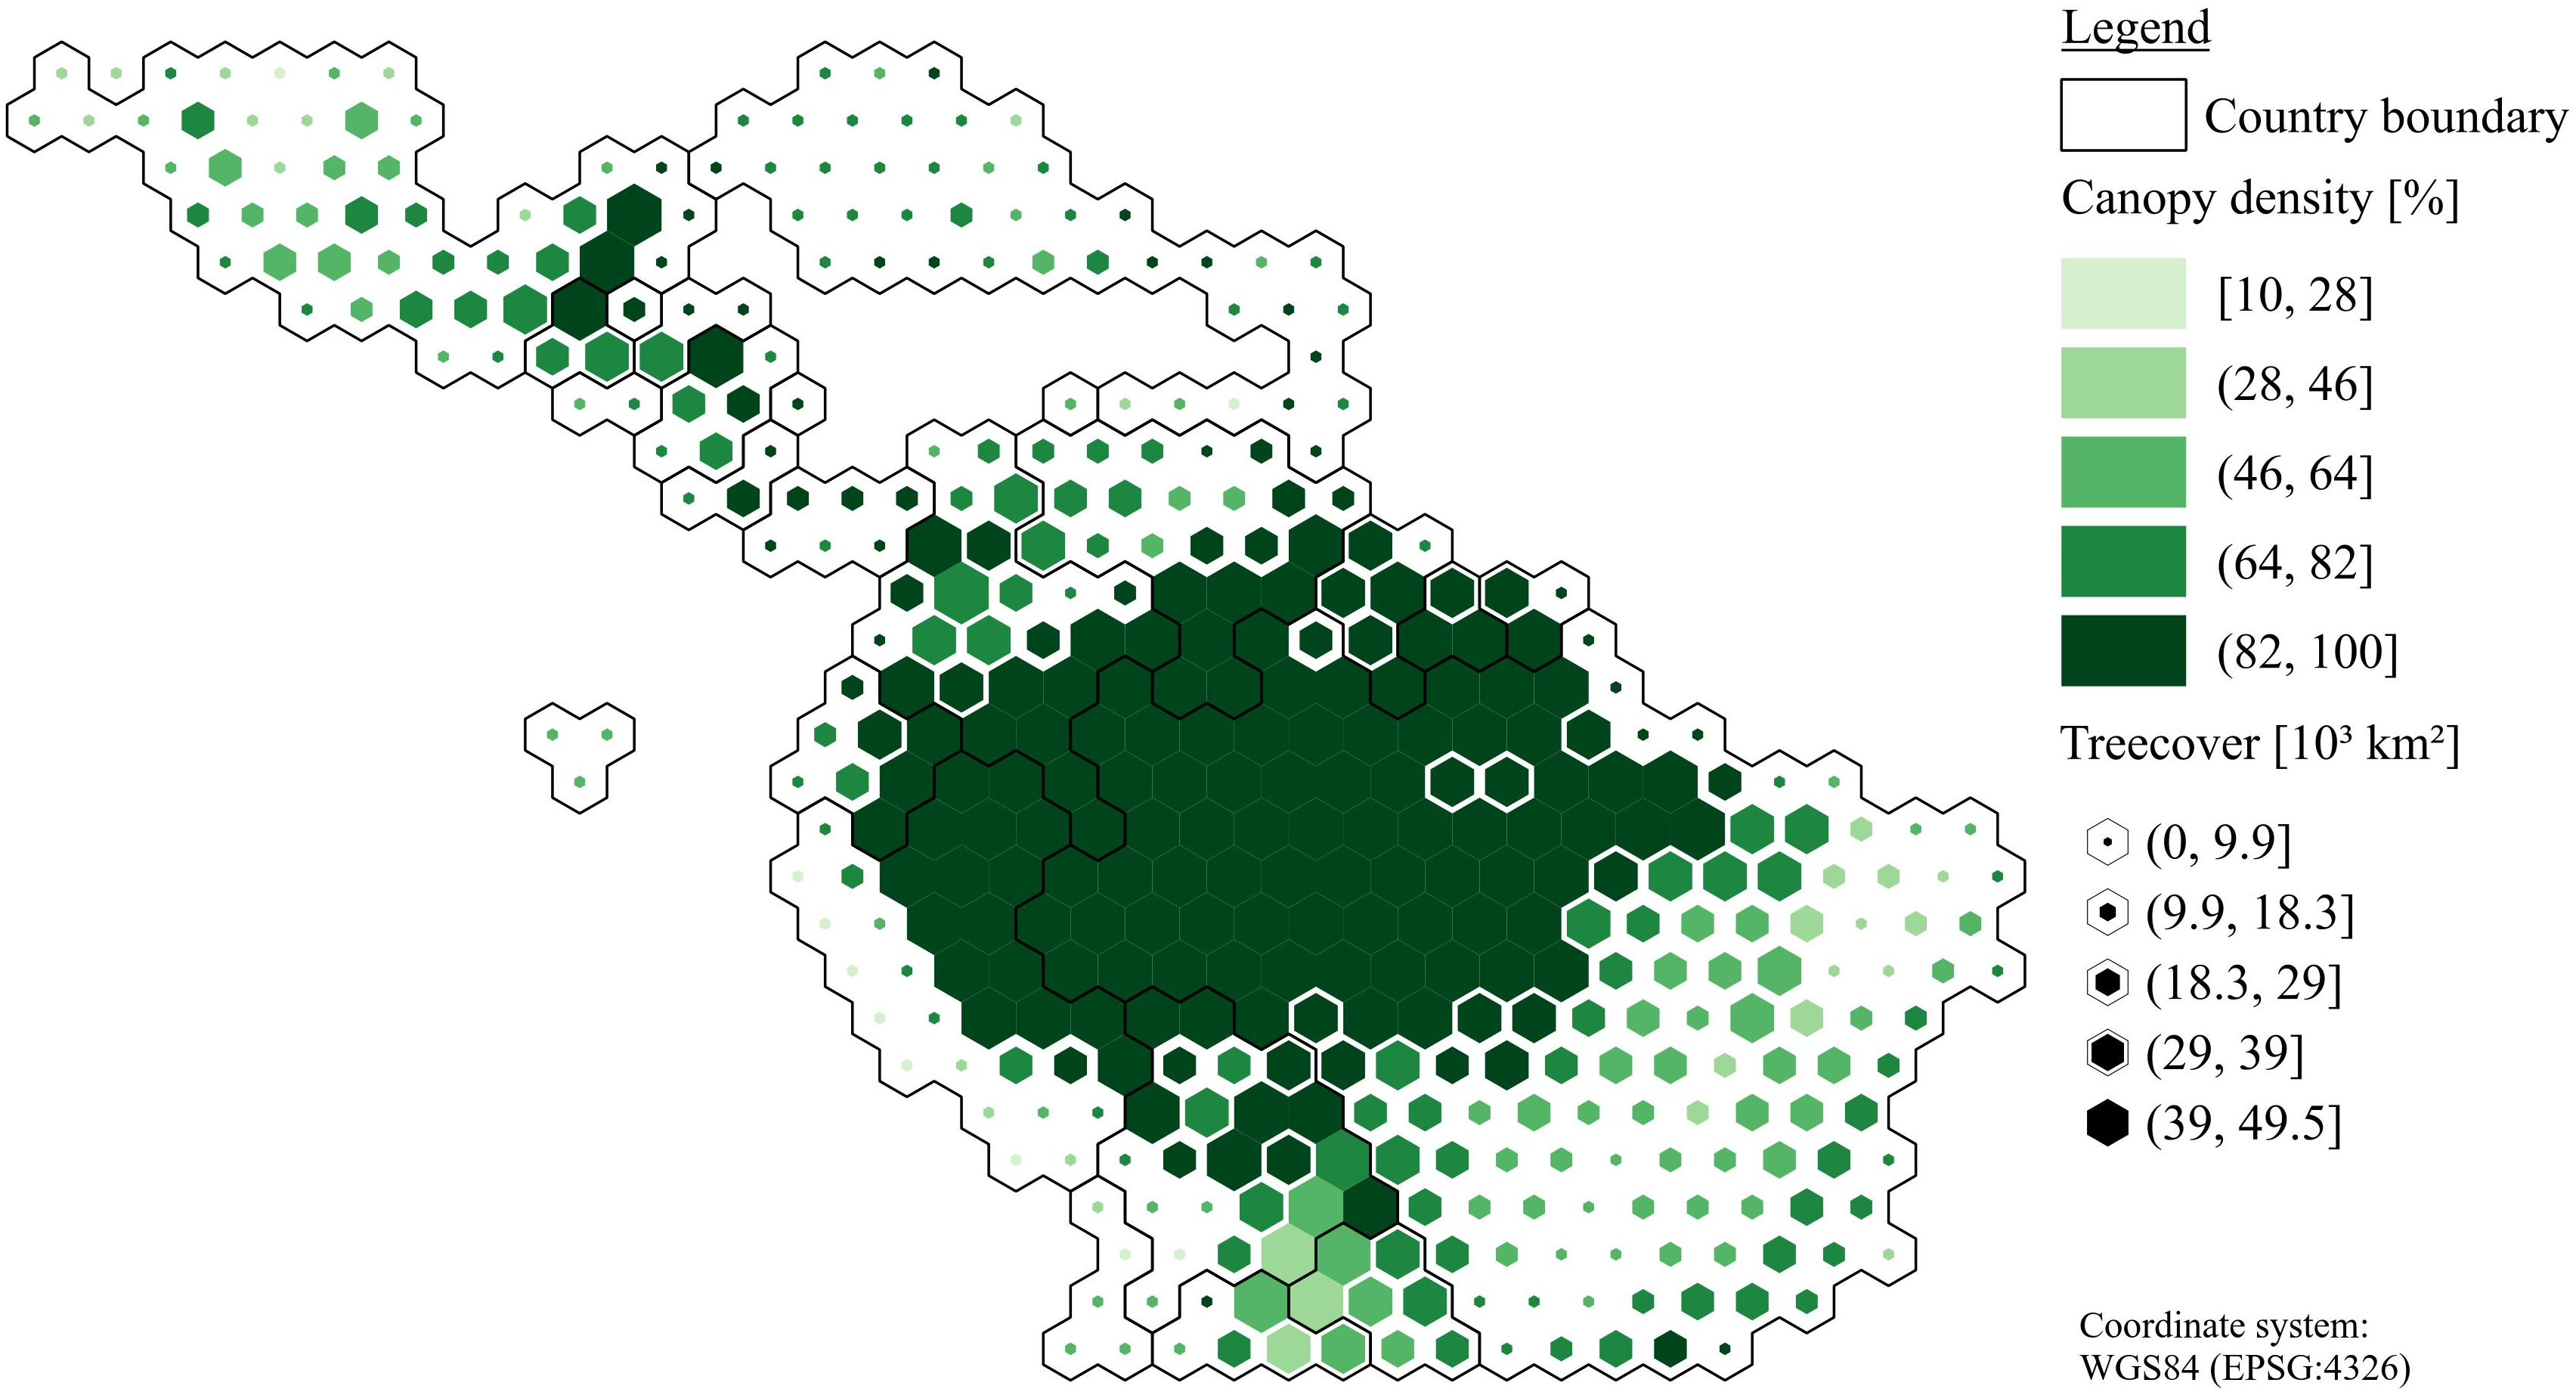
\includegraphics[scale=.9]{img/americas_treecover_frameless}
				\caption[Tree cover and canopy density in Latin America at 2000]{\textbf{Tree cover and canopy density in Latin America at 2000:} This map shows the tree cover and mean canopy density distribution at 2000. An unscaled hexagon covers an area of 0.5 decimal degrees which translates to an area of approximately 49 thousand km$^2$ at the equator. Tropical rain forest in the center of the map is characterized by a tree cover between approximately 29 and 49 km$^2$ and canopy densities between 82 and 100 \%. The rain forest is surrounded by tropical moist forest with tree cover up to 49 km$^2$ but lower mean canopy densities between 10 and 82 \% as the rain forest. The tropical dry forest also known as Gran Chaco is located in the lower left of the map distributed over the countries Bolivia, Paraguay, and Argentina.}
				\label{fig:americas_tree_cover}
			\end{figure}

			The figure \ref{fig:americas_loss} shows the distribution of tree cover losses over Latin America within the time frame of 2001 till 2010. During this period an area of approximately 388 thousand km$^2$ was deforested as table \ref{tab:proximate_driver} in the appendix \ref{ch:appendix_c} shows. We could identify for several countries deforestation hot-spots where the deforested area is between approximately 2.7 and 9 thousand km$^2$ as the map suggests. Tropical countries with deforestation hot-spots are: Paraguay, Argentina, Bolivia, Brazil, Colombia, Peru, and Guatemala. In Brazil the hot-spots of tree cover loss are known as arc of deforestation and cover the states of Acre, Rond\^{o}nia, Mato Grosso, and Pará while the deforestation starts to move into the state of Amazonas \citep{Wood2002}. The tree cover loss within this arc develops along the highway network in this regions \citep{Alves2002,Mueller2016}. Several paved highways like BR-163, BR-219, BR-230 etc. foster the agricultural and infrastructural development and lead to high deforestation rates. In Brazil an area of approximately 274 thousand km$^2$ is deforested between 2001 and 2010. Deforestation hot-spots in Paraguay and Argentina are located in the Gran Chaco region which was one of the least disturbed forests worldwide and is exposed to high deforestation rates since 1969 \citep{Caldas2013,Zak2004}. During our study time frame deforestation accounts for an area of approximately 7097 km$^2$ and 21 thousand km$^2$ in the Chaco region in Argentina and Paraguay, respectively. In Bolivia the deforestation hot-spot is located in the department of Santa Cruz. Bolivia had till the 1960s relative low deforestation rates which increased moderately after and increased sharply during the 1990s and remain high as the map suggests \citep{Pacheco2002,DavidKaimowitz2002}. During the first decade of 2000 an area of approximately 19 thousand km$^2$ is exposed to tree cover loss. The department of Petén in Guatemala is committed to deforestation since the 1980s \citep{Beach1998}. Since 2000 the deforestation rates in Guatemala are among the highest in Latin America and after 2005 the rates increased further \citep{McSweeney2014}. During 2001 and 2010 an area of approximately 6515 km$^2$ is exposed to tree cover loss as table \ref{tab:proximate_driver} shows. \citeauthor{McSweeney2014} highlights that deforestation hot-spots often spatially overlap with drug trafficking nodes. Especially in the department of Petén where large ranches are owned by narco-traffickers. In Peru deforestation hot-spots covering the provinces of Huánuco, Loreto, San Martin, and Ucayali, while the cumulative forest loss account for an area of approximately 8 thousand km$^2$ in the entire country. An area of approximately 15 thousand km$^2$ is exposed to deforestation in Colombia, while deforestation hot-spots are located in Cacquetá, Bolívar, and Antioquia.
			\begin{figure}[ht]
				\centering
				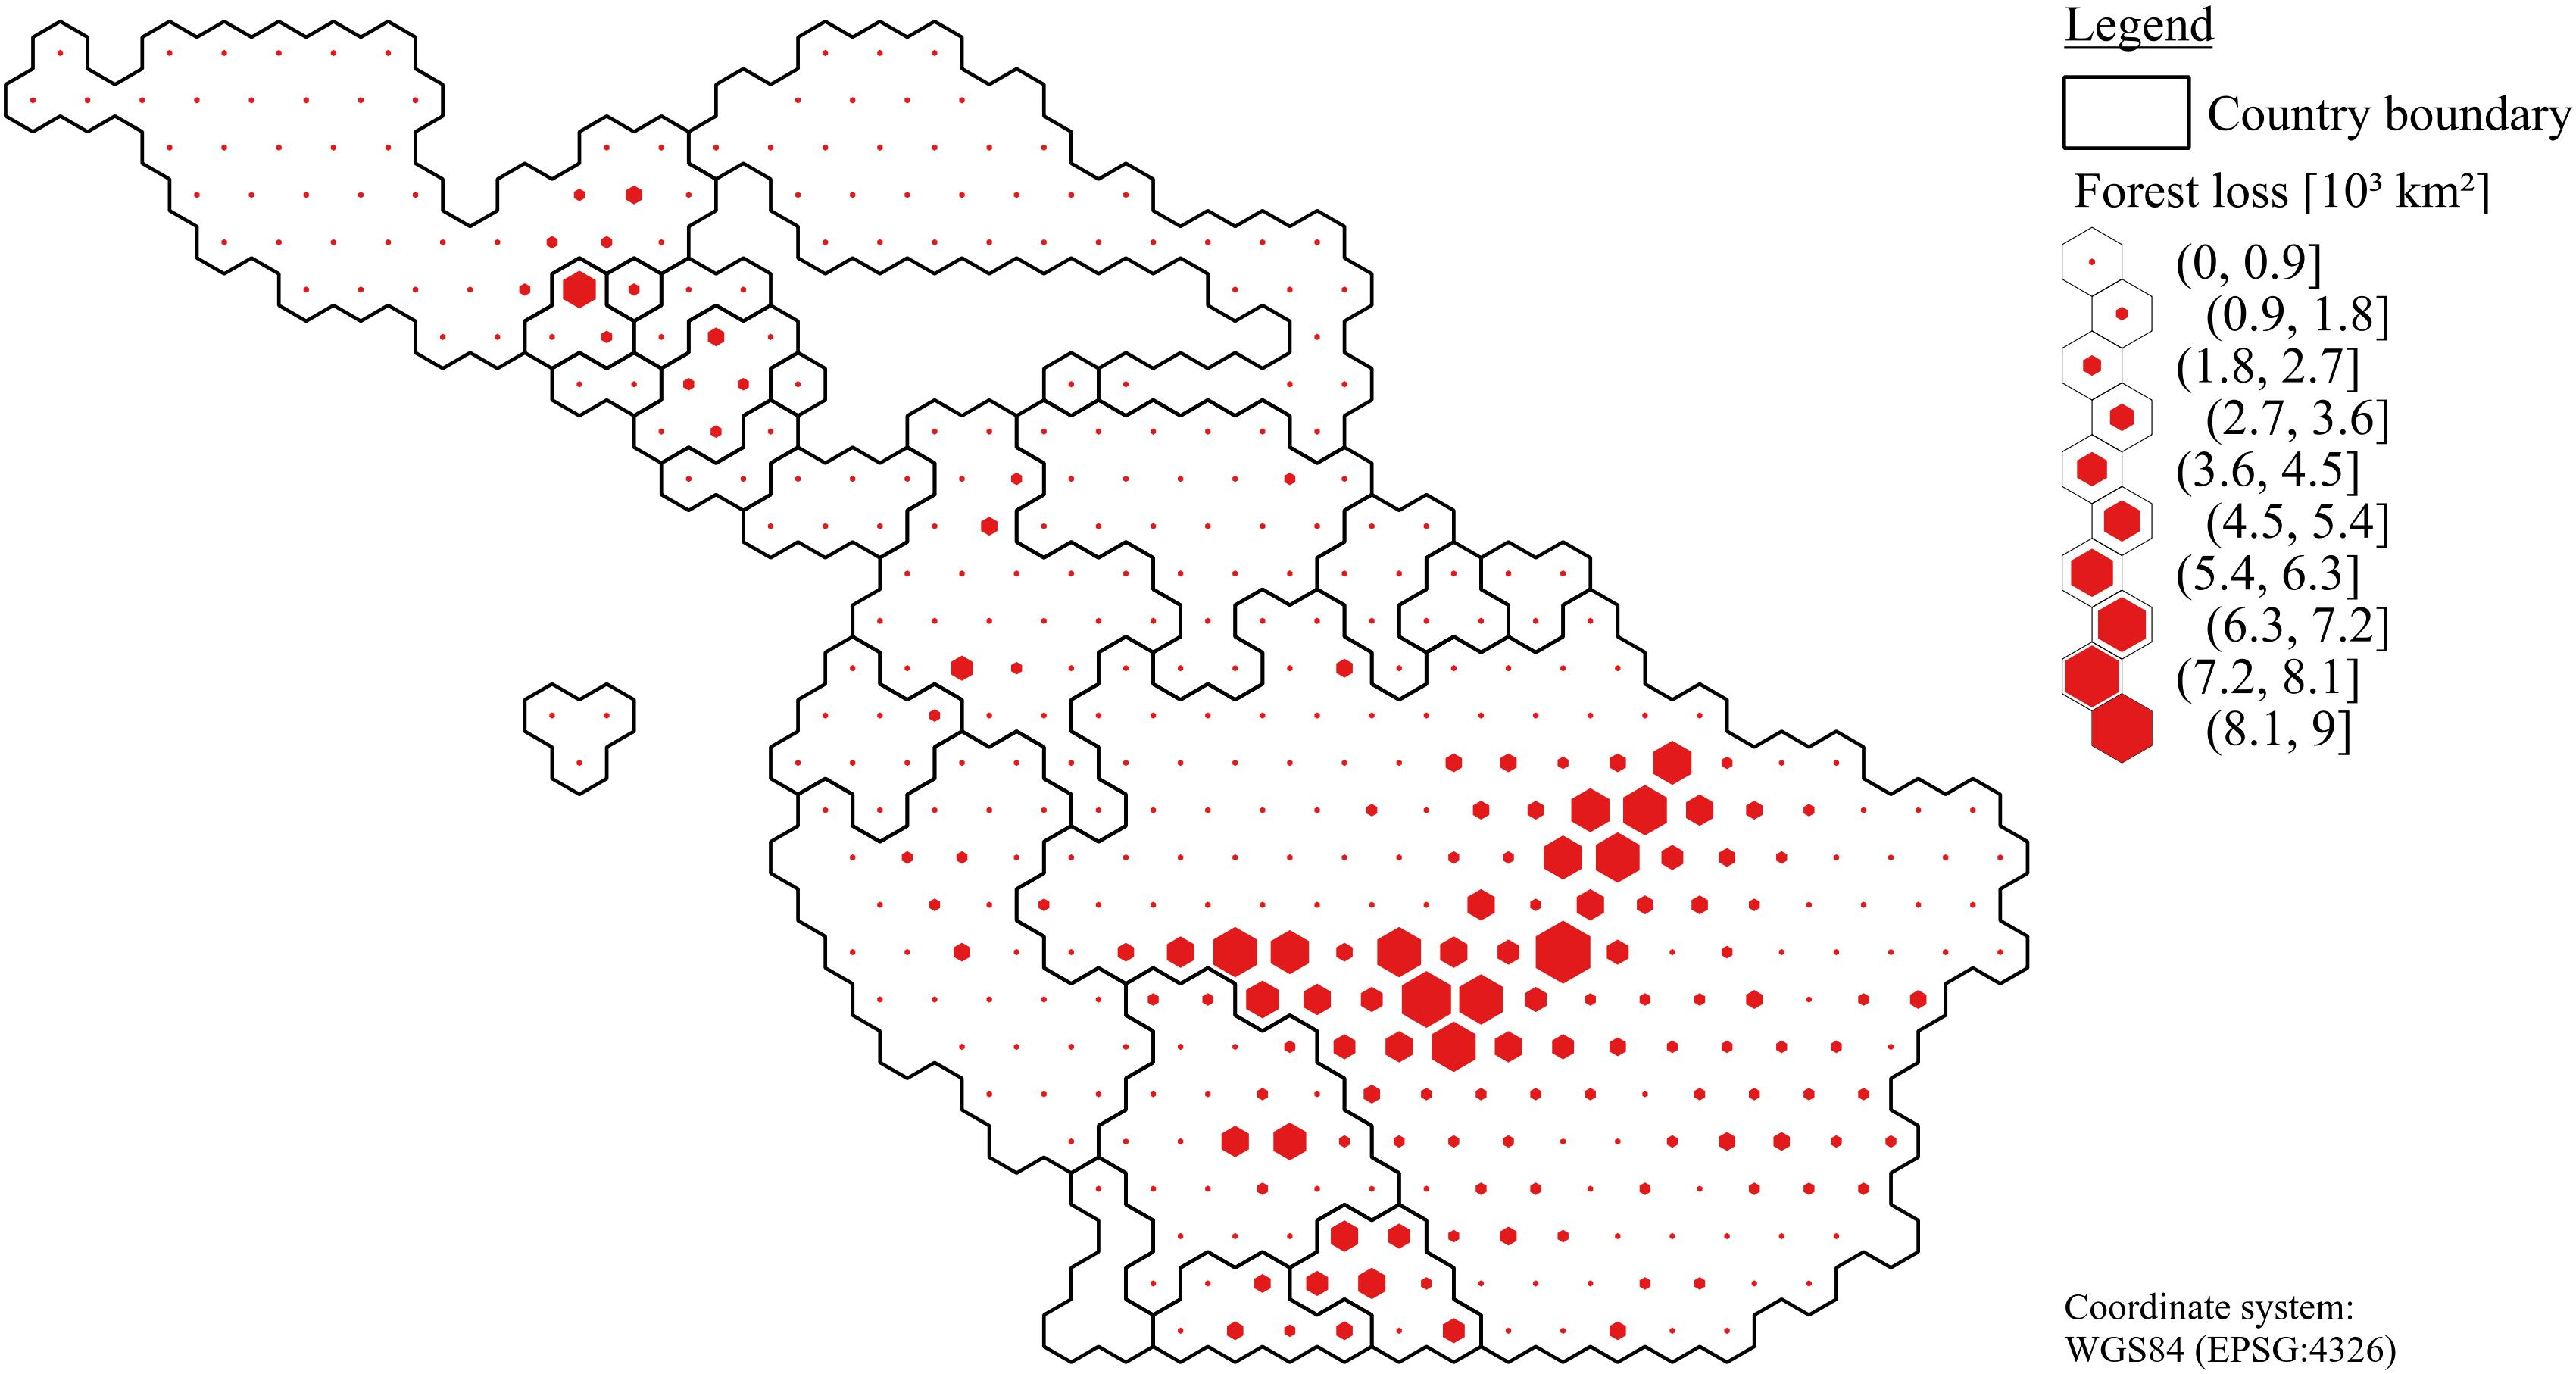
\includegraphics[scale=.9]{img/americas_loss_frameless}
				\caption[Tree cover loss in Latin America between 2001 and 2010]{\textbf{Tree cover loss in Latin America between 2001 and 2010:} This map shows the tree cover loss within our study extent between 2001 and 2010. An unscaled hexagon covers an area of 0.5 decimal degrees which translates to an area of approximately 49 thousand km$^2$ at the equator. Deforestation hot-spots with tree cover loss about 2.7 thousand km$^2$ per hexagon are located in Paraguay, Argentina, Bolivia, Brazil, Colombia, Peru, and Guatemala.}
				\label{fig:americas_loss}
			\end{figure}

			The map in figure \ref{fig:asia_tree_cover} shows the tree cover and canopy density distribution for Asia/Australia. In Asia the tropical rain forest is distributed over several southeast Asian islands like the Indonesian islands Sumatra, Borneo, Java, Papua etc., the Philippines, Malaysia, and Papua New Guinea. Generally the rain forest is characterized by high tree covers comparable to Latin America but in our map most of the islands are smaller than a single hexagon. Therefore, by our method to compute the hexagon scaling the size of the polygons don't reflect the tree cover as share of the landmass and most of them appear smaller. The mean canopy density of tropical rain forest is between 82 and 100 \% and the tree cover is above approximately 9.9 km$^2$. Tropical moist and dry forest are distributed over the continental Asia covering the countries India, Vietnam, Cambodia, Laos etc. These forests are characterized lower tree cover among 9.9 km$^2$ and canopy densities between 10 and 82 \% while the lower tree cover indicates that in southeast Asia deforestation occurs since the 1950s \citep{Kummer1994}. 
			\begin{figure}[ht]
				\centering
				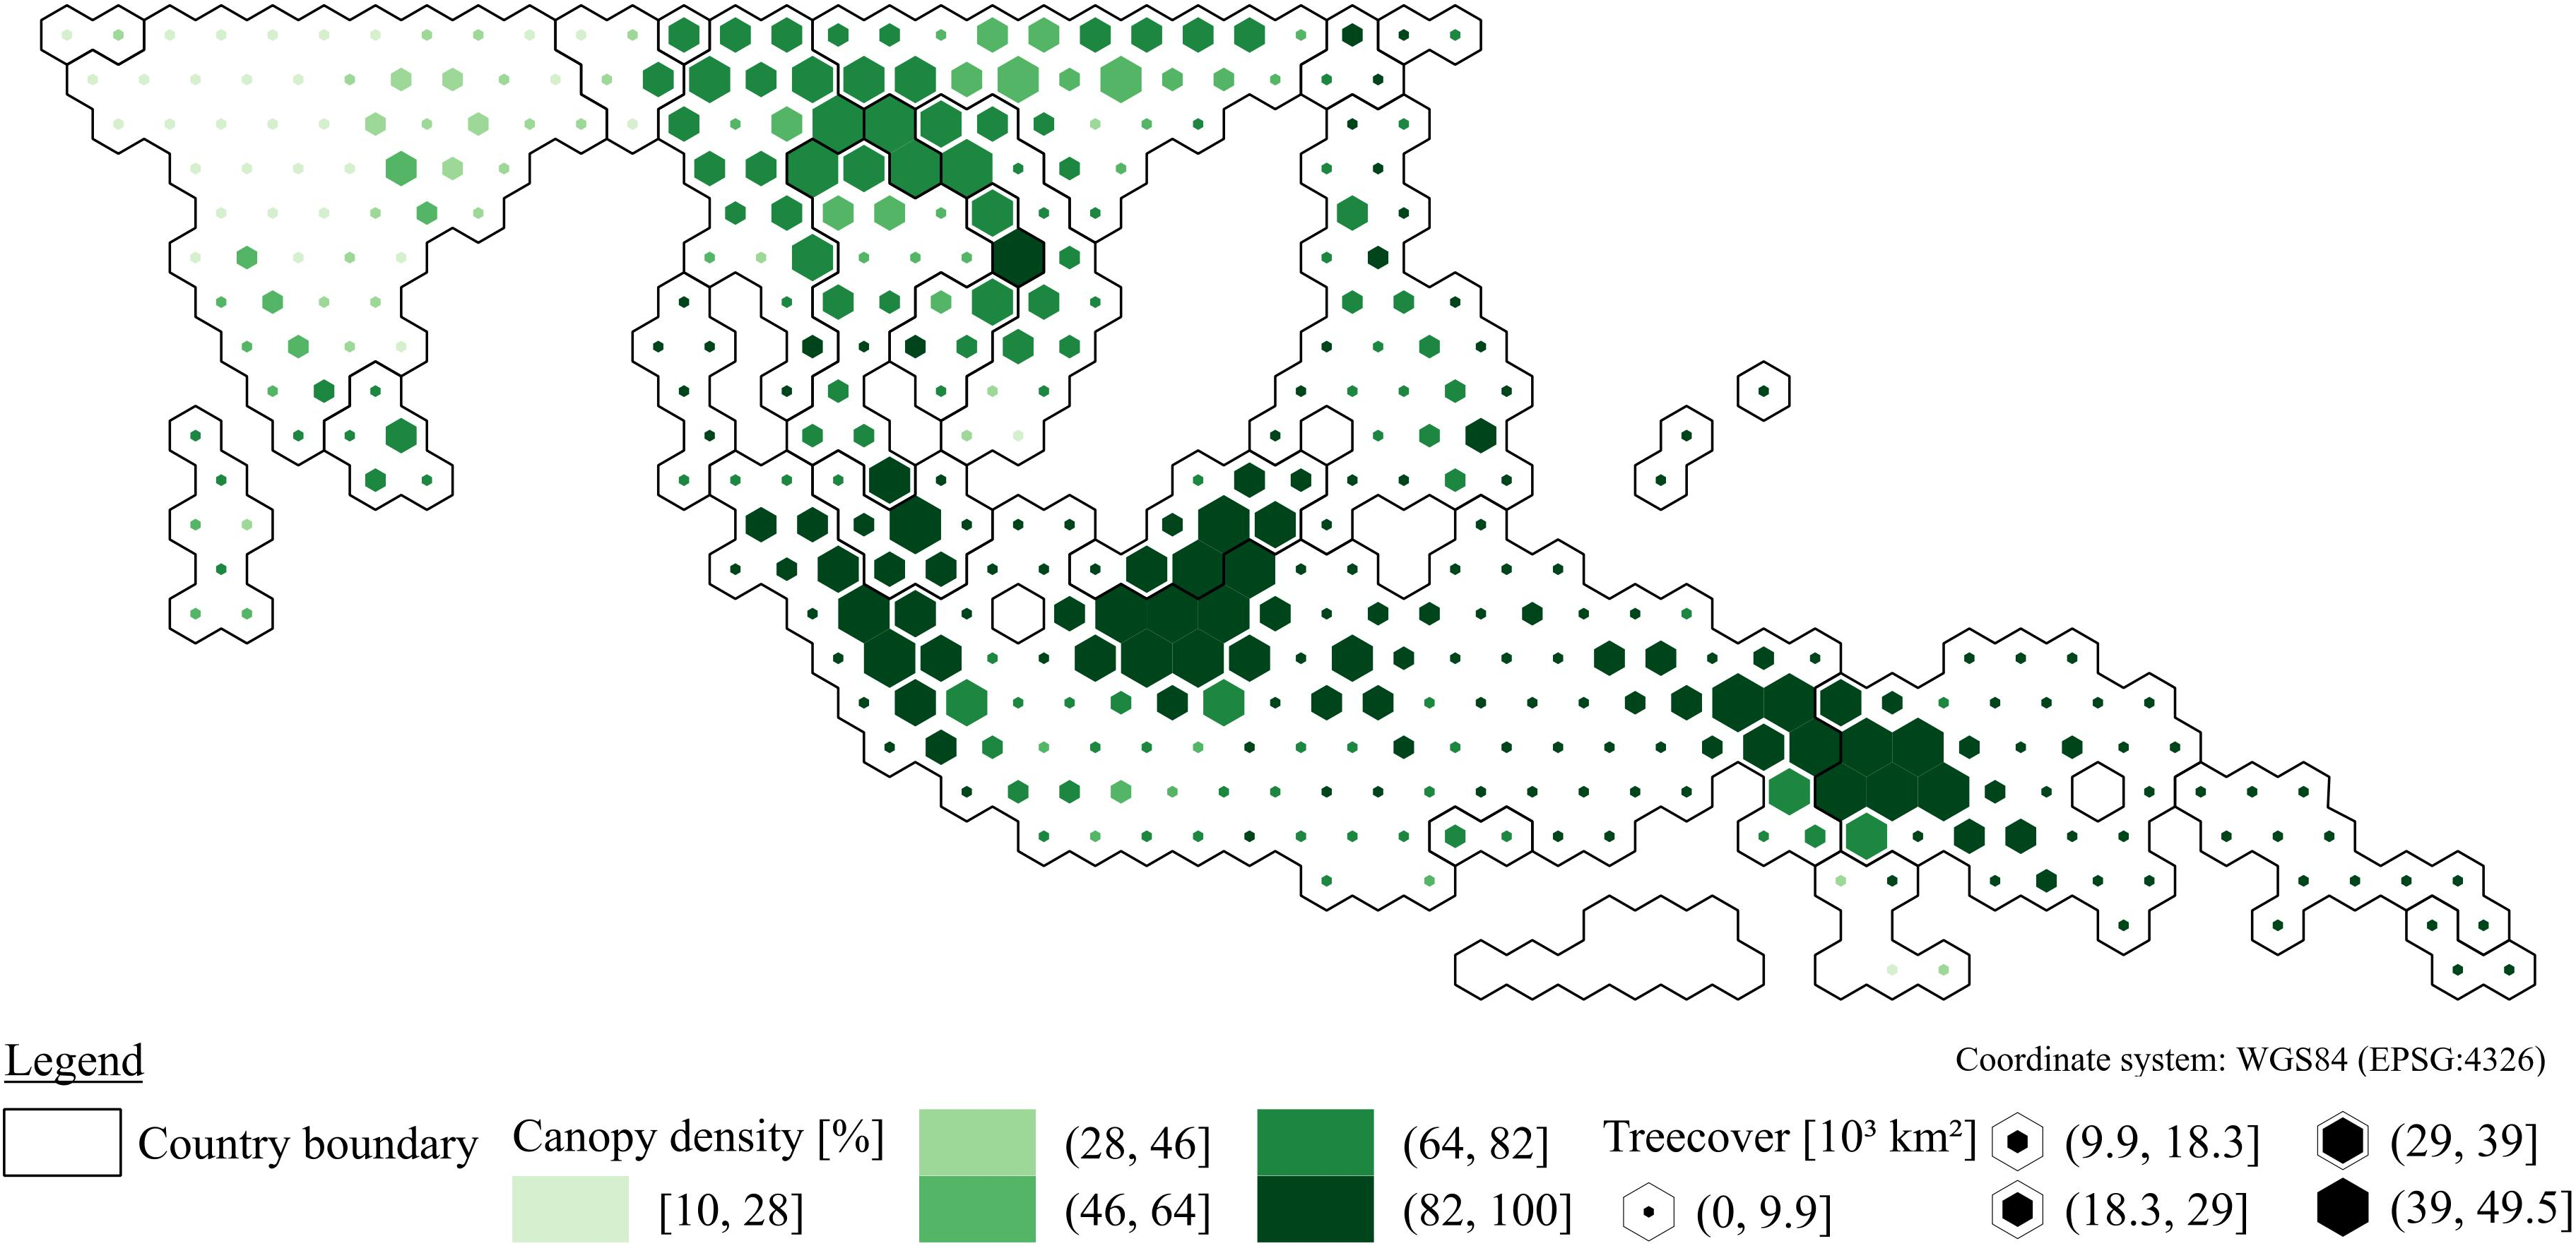
\includegraphics[scale=.9]{img/asia_treecover_frameless}
				\caption[Tree cover and canopy density in Asia/Australia at 2000]{\textbf{Tree cover and canopy density in Asia/Australia at 2000:} This maps shows the tree cover and mean canopy density distribution within our study extent at 2000. An unscaled hexagon covers an area of 0.5 decimal degrees which translates to an area of approximately 49 thousand km$^2$ at the equator.}
				\label{fig:asia_tree_cover}
			\end{figure}

			The map in figure \ref{fig:asia_loss} shows the distribution of tree cover loss in Asia/Australia for the time period 2001 till 2010. During this period a forest area of approximately 196 thousand km$^2$ is exposed to deforestation as table \ref{tab:proximate_driver} in the appendix \ref{ch:appendix_c} suggests. For this region we identified the following countries as deforestation hot-spots with deforestation areas per hexagon of approximately 1.9 to 9 thousand km$^2$: Indonesia, continental and insular Malaysia, Vietnam, and Laos. Indonesia is known as a country with one of the highest rates of primary forest loss for the time period 2000 till to 2016 \citep{Austin2019}. In the first decade of 2000 an area of approximately 100 thousand km$^2$ is exposed to deforestation as table \ref{tab:proximate_driver} suggests. Tree cover loss is predominantly distributed over the Indonesian islands of Sumatra and Borneo (Kalimantan) as the map \ref{fig:asia_loss} shows. Indonesia's forests are exposed to deforestation by dynamic causes since the 1950s \citep{Nawir2007}. Malaysia has lost an area of approximately thousand 33 km$^2$ by deforestation during the time frame 2001 till 2010. The deforestation hot-spots in Malaysia are distributed over the Malaysian Borneo (Sarawak/Sabah) and the continental Malaysia. Comparable to Indonesia, Malaysia's forests are exposed to deforestation since the 1950s by dynamic causes like logging followed by agricultural activities \citep{Kummer1994}. From 2001 till 2010 an area of approximately thousand km$^2$ was exposed to deforestation in Vietnam as table \ref{tab:proximate_driver} suggests. We identified the central highland provinces Dak Lak, Dak Nong, Gia Lai, and Lam Dong as deforestation hot-spots. \citet{Meyfroidt2013} confirms this in his study on trajectories of deforestation and highlights that the losses in this area could reduce the benefits of national-scale forest recovery. During the early 1990s a transition to reforestation was encouraged and natural forests expanded in Vietnam but it is connected with a increased loss in the highland regions \citep{Meyfroidt2013,Chazdon2008}. In Laos a forest area of approximately 8 thousand km$^2$ is lost during the time period 2001 till 2010. The map in figure \ref{fig:asia_loss} suggests that northern Laos is predominantly exposed to tree cover loss while \citet{Hirsch2000} confirms. Laos is known for a steady loss of forest cover since the early 1960s. Whereas the causes for this \ac{LC} transitions are dynamically changing till now.
			\begin{figure}[ht]
				\centering
				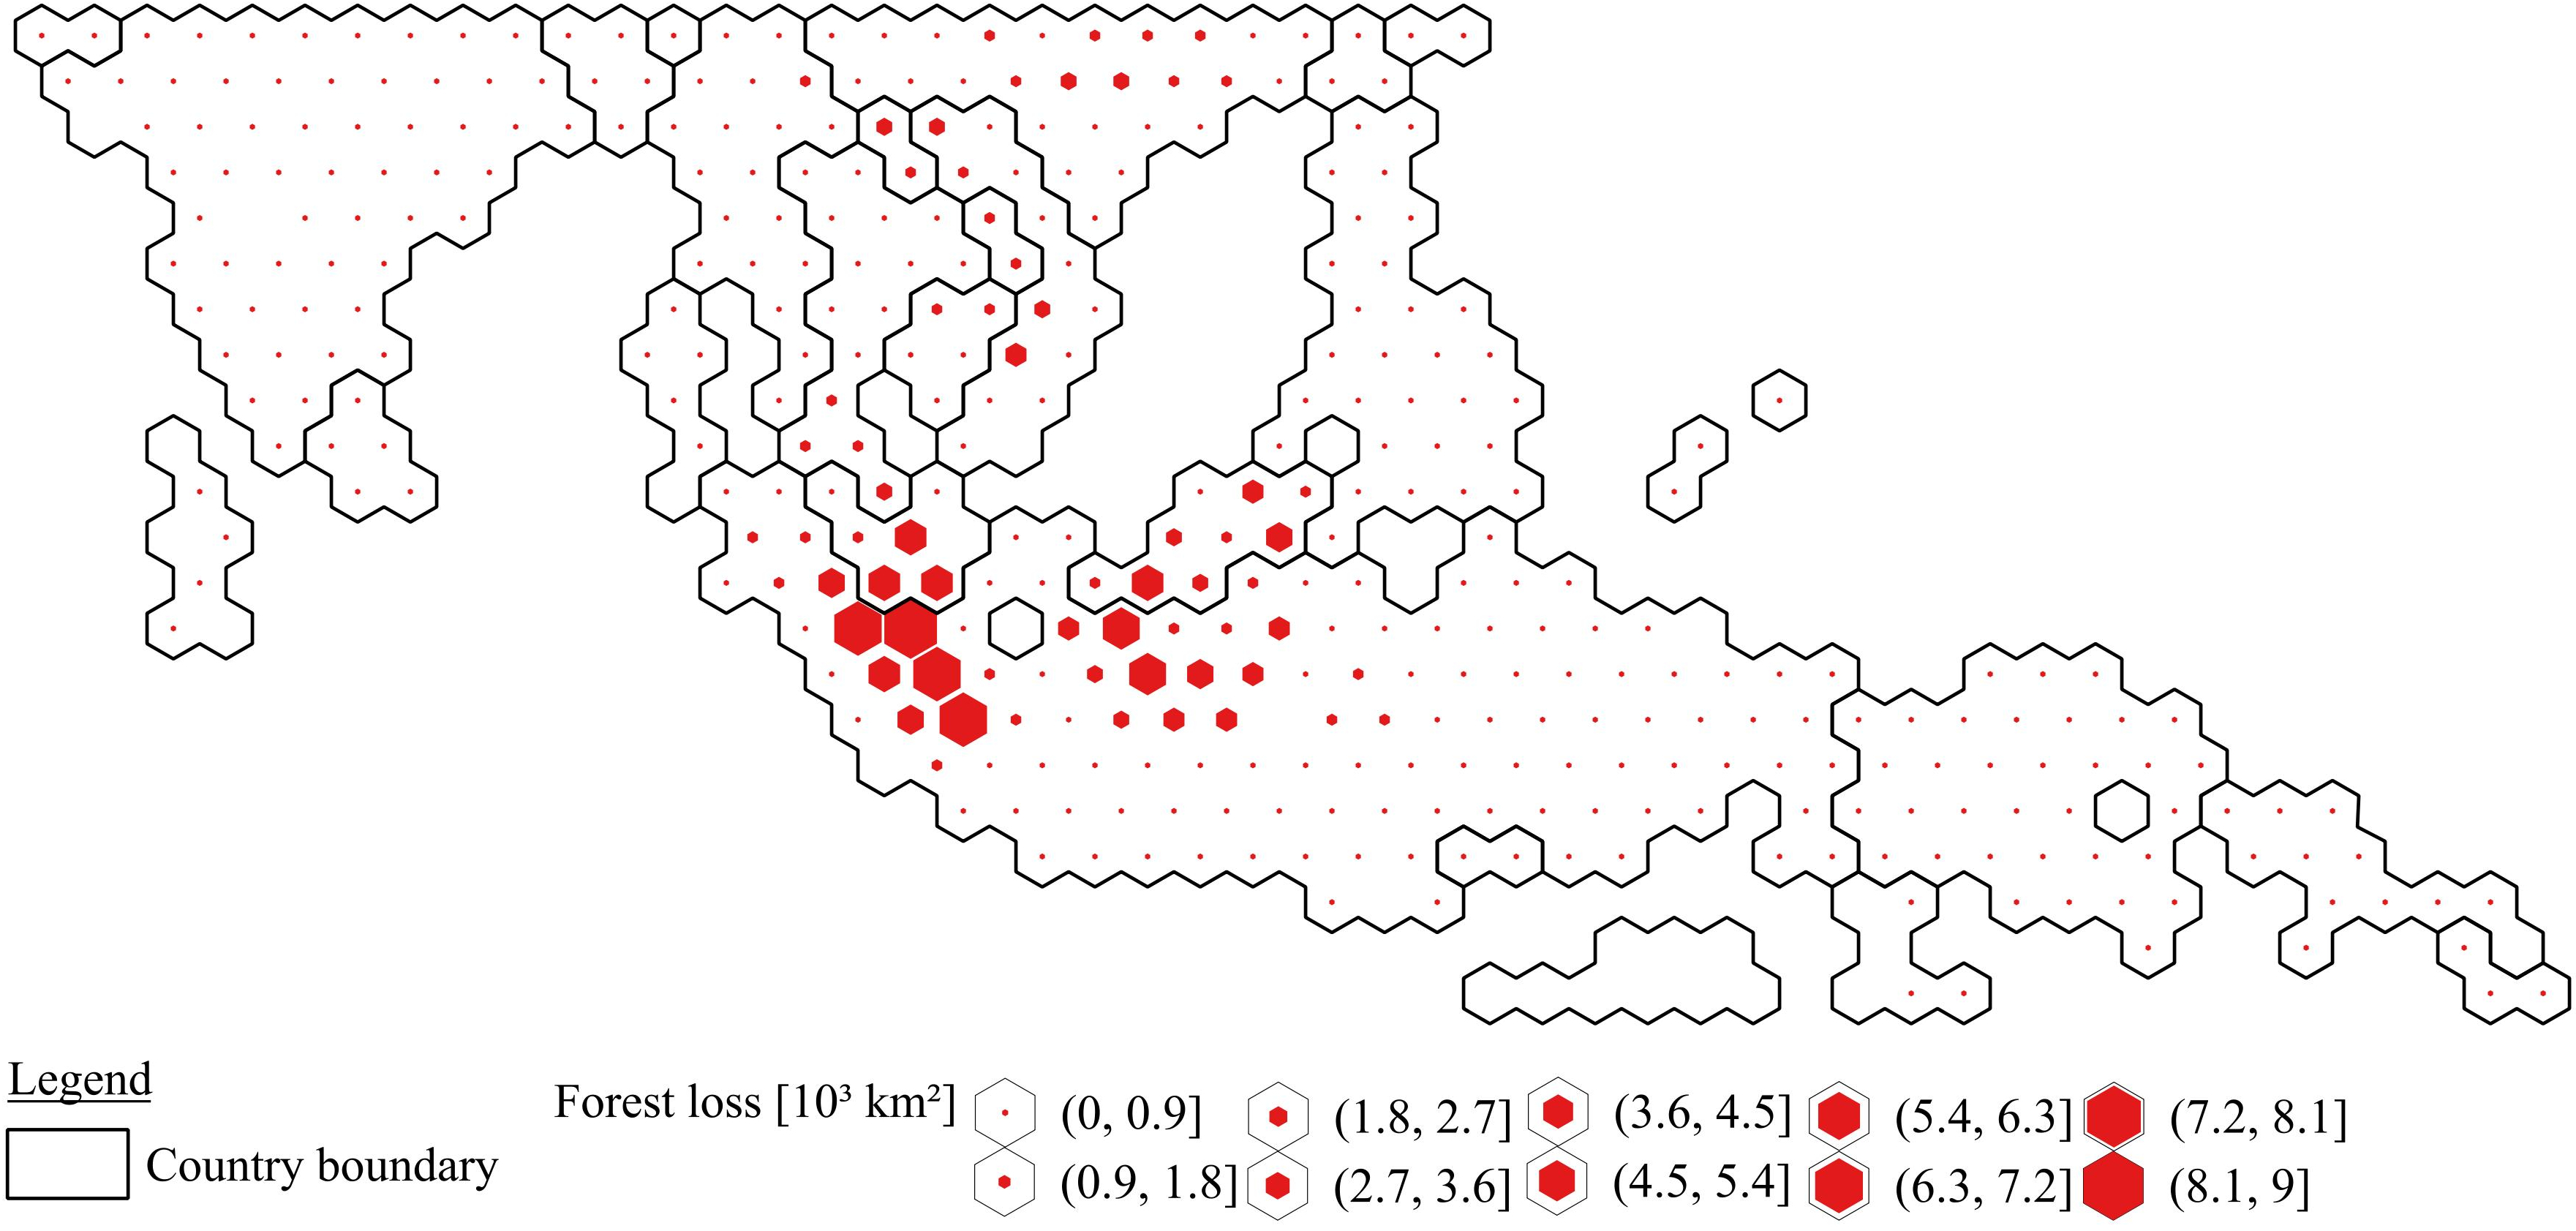
\includegraphics[scale=.9]{img/asia_loss_frameless}
				\caption[Tree cover loss in Asia/Australia between 2001 and 2010]{\textbf{Tree cover loss in Asia/Australia between 2001 and 2010:} This map shows the tree cover loss within our study extent between 2001 and 2010. An unscaled hexagon covers an area of 0.5 decimal degrees which translates to an area of approximately 49 thousand km$^2$ at the equator. Deforestation hot-spots with tree cover loss about 1.9 thousand km$^2$ per hexagon are located in Indonesia, Malaysia, Vietnam, and Laos.}
				\label{fig:asia_loss}
			\end{figure}

			Figure \ref{fig:africa_tree_cover} shows the tree cover and canopy density distribution over Africa. In Africa the tropical rain forest is distributed over the following central African countries: Democratic Republic of the Congo, Republic of the Congo, Equatorial Guinea, Gabon, Cameroon, and partial in Ghana, Ivory Coast, and Liberia. In our map this type of forest is characterized by a dense tree cover between 39 and 49 thousand km$^2$ per hexagon while the canopy density between 64 and 100 \% does not separate it from the moist type as good as in Latin America and Asia/Australia. The rain forest is surrounded by tropical moist forest with a dense tree cover between 18 and 49 thousand km$^2$ while the mean canopy density between 10 and 82 \% is sparser then tropical rain forest. Countries covered by the moist tropical forest type are the following examples: Angola, Uganda, Central African Republic, Zambia, Madagascar etc. Tropical dry forest is characterized by a sparse tree cover among approximately 18 thousand km$^2$ per hexagon and canopy densities between 10 and 46 \%. Mozambique, Tanzania, and Nigeria are examples for countries covered partial by tropical dry forest.
			\begin{figure}[ht]
				\centering
				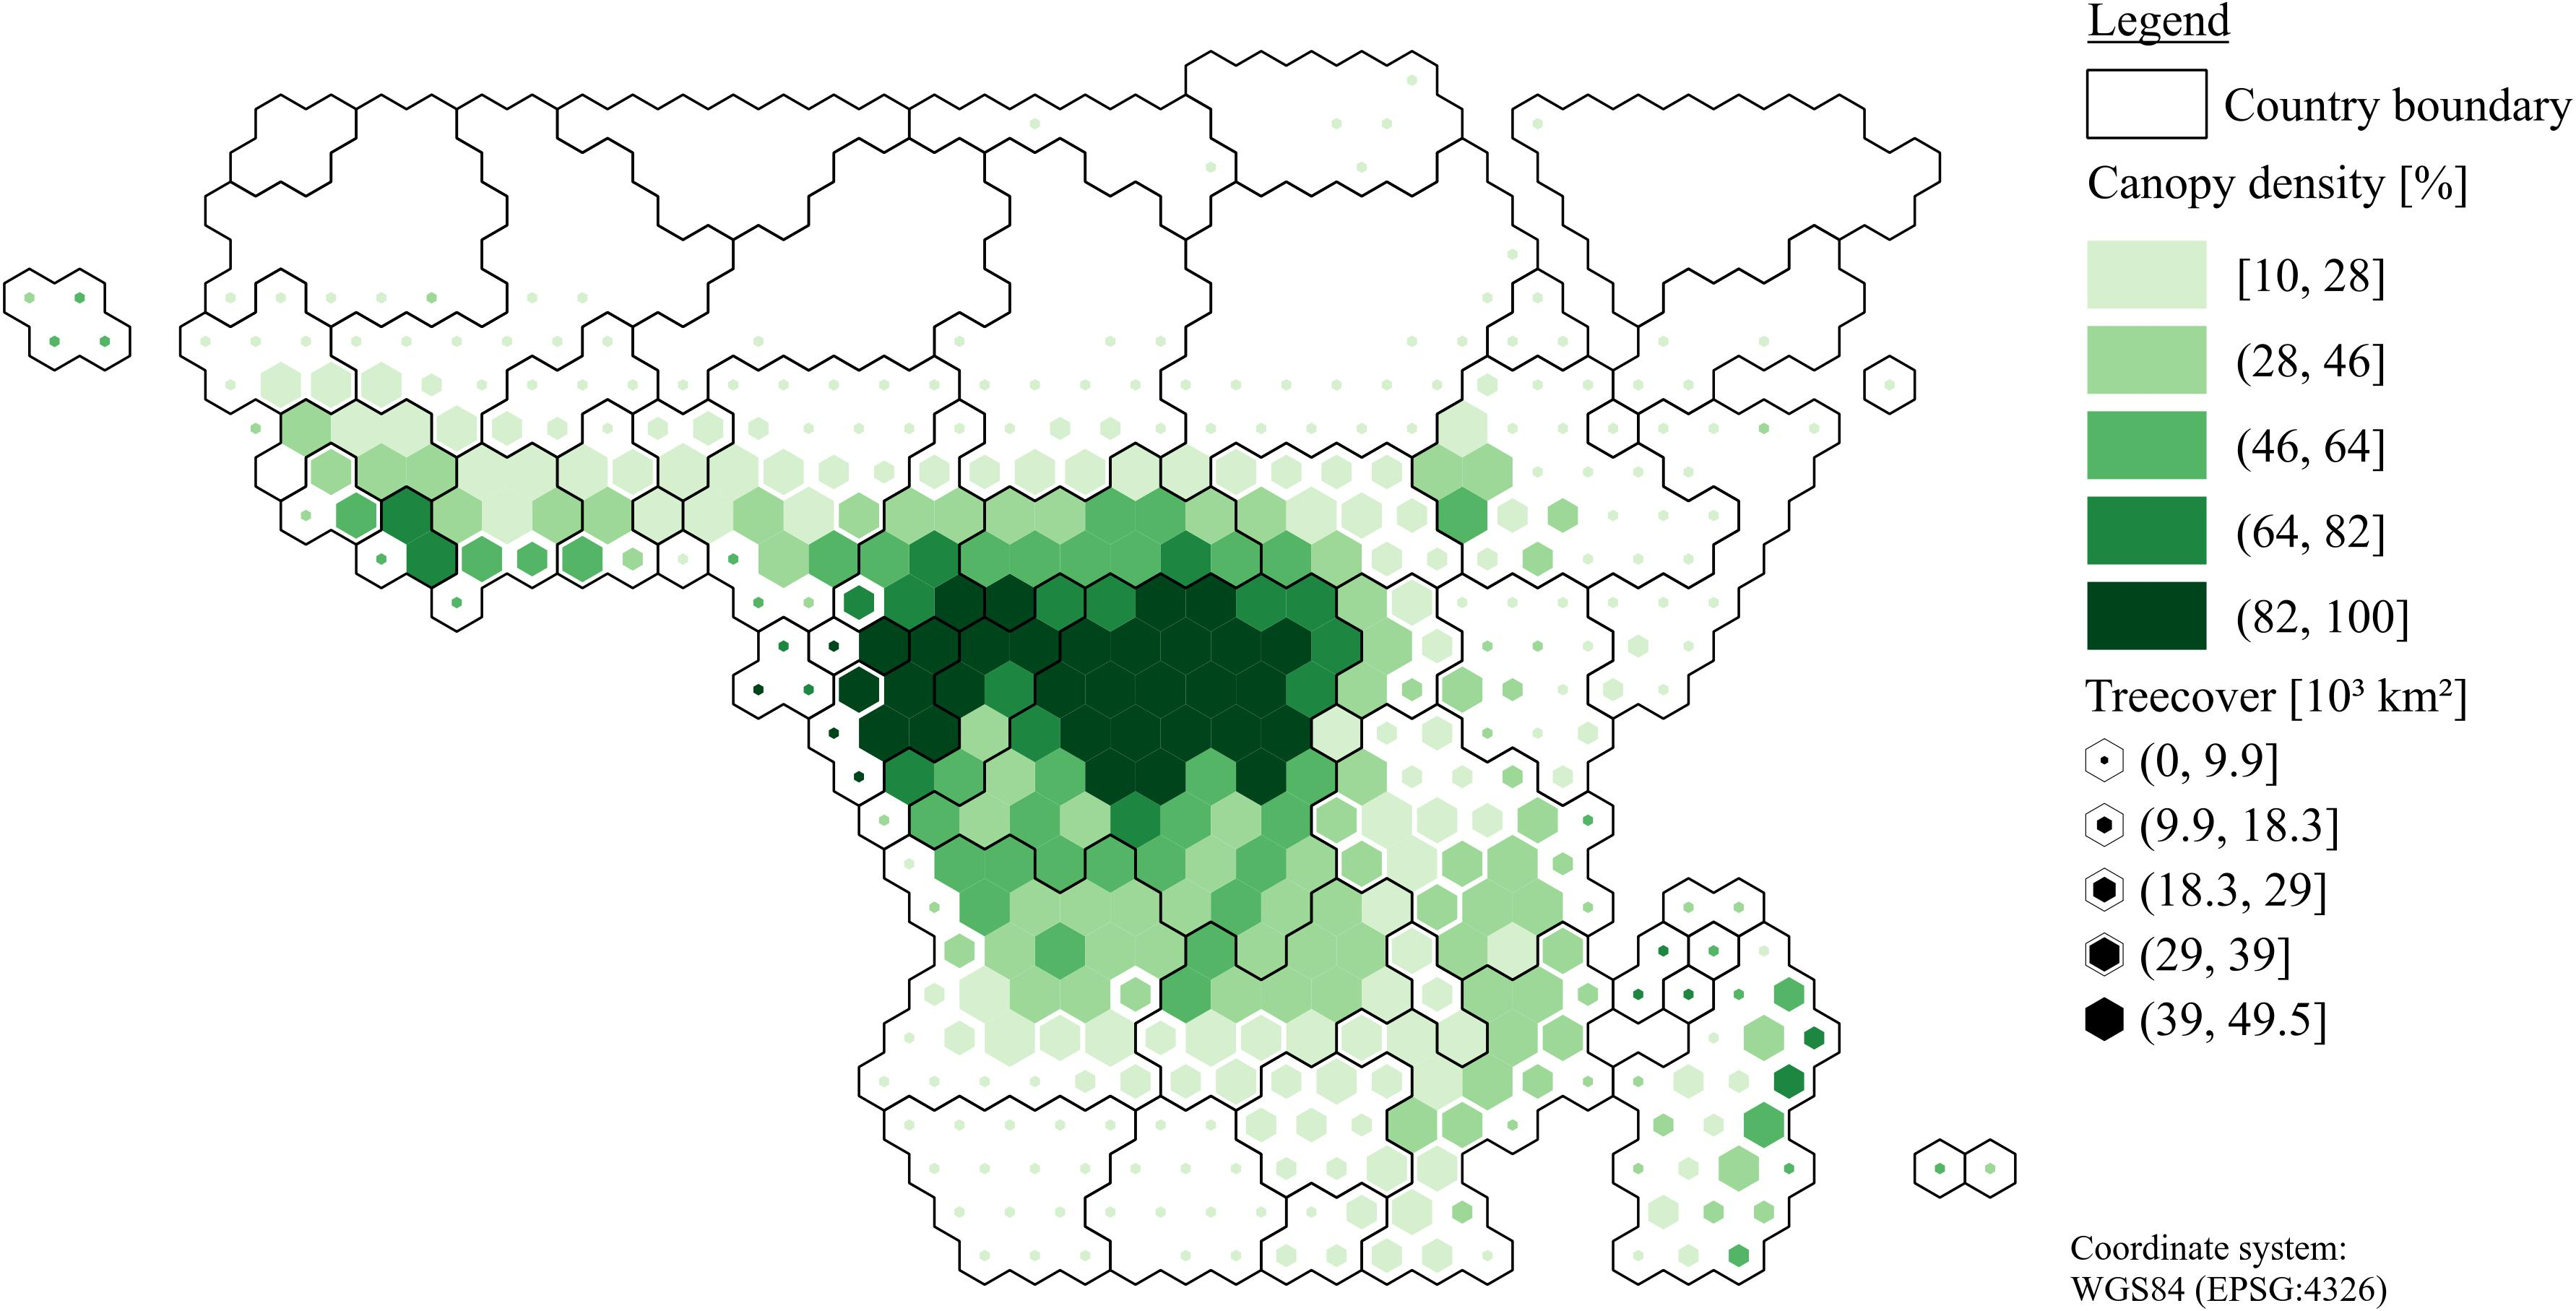
\includegraphics[scale=.9]{img/africa_treecover_frameless}
				\caption[Tree cover and canopy density in Africa at 2000]{\textbf{Tree cover and canopy density in Africa at 2000:} This maps shows the tree cover and mean canopy density distribution within our study extent at 2000. An unscaled hexagon covers an area of 0.5 decimal degrees which translates to an area of approximately 49 thousand km$^2$ at the equator. Tropical rain forest is characterized by dense tree cover between 39 and 49 thousand km$^2$ and high canopy density above 64 \% in the center of Africa. The rain forest is surrounded by tropical moist forest with a dense tree cover as well but a lower mean canopy density between 10 and 82 \%.}
				\label{fig:africa_tree_cover}
			\end{figure}

			The map in figure \ref{fig:africa_loss} shows the regions which are exposed to tree cover loss in Africa for the time period 2001 till 2010. During the first decade of 2000 an area of approximately 174 km$^2$ was deforested as table \ref{tab:proximate_driver} in the appendix \ref{ch:appendix_c} suggests. With tree cover loss between 1.1 and 3.7 thousand km$^2$ per hexagon we identified the following countries as deforestation hot-spots: Ivory Coast, Democratic Republic of the Congo, Angola, Mozambique, Madagascar, and Tanzania. At the Ivory Coast an area of approximately 10 thousand km$^2$ was exposed to deforestation between 2001 and 2010 as table \ref{tab:proximate_driver} shows. The map in figure \ref{fig:africa_loss} shows that the deforestation hot-spots are located in the southern and northern parts of the country. Evidences for this are given by \citet{Goetze2006} and \citet{Barima2016}. Lower deforestation in the center of the country can be explained by a military conflict started in 2002 that divides the country in a northern and southern zone with a buffer zone in between controlled by Un forces and French soldiers \citep{Barima2016}. At the Ivory coast continuous loss of tree cover by deforestation started approximately in the 1958s \citep{Chatelain1996}. The deforestation accounts for an area of approximately 45 thousand km$^2$ in the Democratic Republic of the Congo. The DR Congo home of the second largest tropical forest in the world has compared to other tropical countries relatively low deforestation dynamics but recent studies show that deforestation could accelerate in the future \citep{Ickowitz2015}. The deforestation hot-spots are located in the eastern Congo and around medium-sized cities along the Congo river in the lower center of the country. During the first decade of the 2000s an area of about 13 thousand km$^2$ is deforested in Angola. Deforestation hot-spots are more oriented to the center of the country covering roughly the provinces Huambo, Bie, and Moxico as the map in figure \ref{fig:africa_loss} suggests. For the time period 1990 till 2009 \citet{Cabral2011} performed a study on forest change in the province of Huambo where a decrease in dense forest cover is observed while the cover of sparse forest is increasing \citep{Cabral2011}. Another study by \citet{Schneibel2017} on deforestation dynamics in south-central Angola reveals that the tree cover loss develops along anthropogenic infrastructure and forests are exploited over a long term until (fuel-wood collection etc.) a \ac{LC} transitions to other types like cropland occurs. To best of our knowledge no studies on historic deforestation dynamics exist for Angola due to the civil war from 1975 till 2002. In Mozambique an area of approximately 18 thousand km$^2$ was exposed to tree cover loss as table \ref{tab:proximate_driver} suggests. During the war between 1976 and 1992 the forests of Mozambique where not largely exposed to deforestation but since end of the war the deforestation rates are increasing \citep{Sitoe2012}. We identified the following provinces as deforestation hot-spots between 2001 and 2010: Zambezia, Nampula, and Cabo Delgado. This is largely confirmed by \citeauthor{Sitoe2012} where it is stated that deforestation is concentrated in the center and north of Mozambique. These hot-spots could be related to the higher population densities within this areas. Tree cover loss accounts for an area of about 11 thousand km$^2$ in Madagascar during the study period. In Madagascar deforestation hot-spots are concentrated at the north-east coast of the island as the map in figure \ref{fig:asia_loss} suggests. Madagascar's central highland forests are exposed to anthropogenic deforestation since 1600, reportedly \citep{Harper2007}. By the nineteenth century the deforestation advanced over the entire island forests. In Tanzania an area of approximately 14 thousand km$^2$ was exposed to tree cover loss. Since the 1900s approximately 19.4 \% of the forest cover is lost \citep{Kideghesho2015}. The map in figure \ref{fig:africa_loss} suggests that deforestation hot-spots are located in the country center covering the following provinces: Lindi, Singida, Tabora, Dodom, Tanga, Pwani, and the island of Zanzibar.
			\begin{figure}[ht]
				\centering
				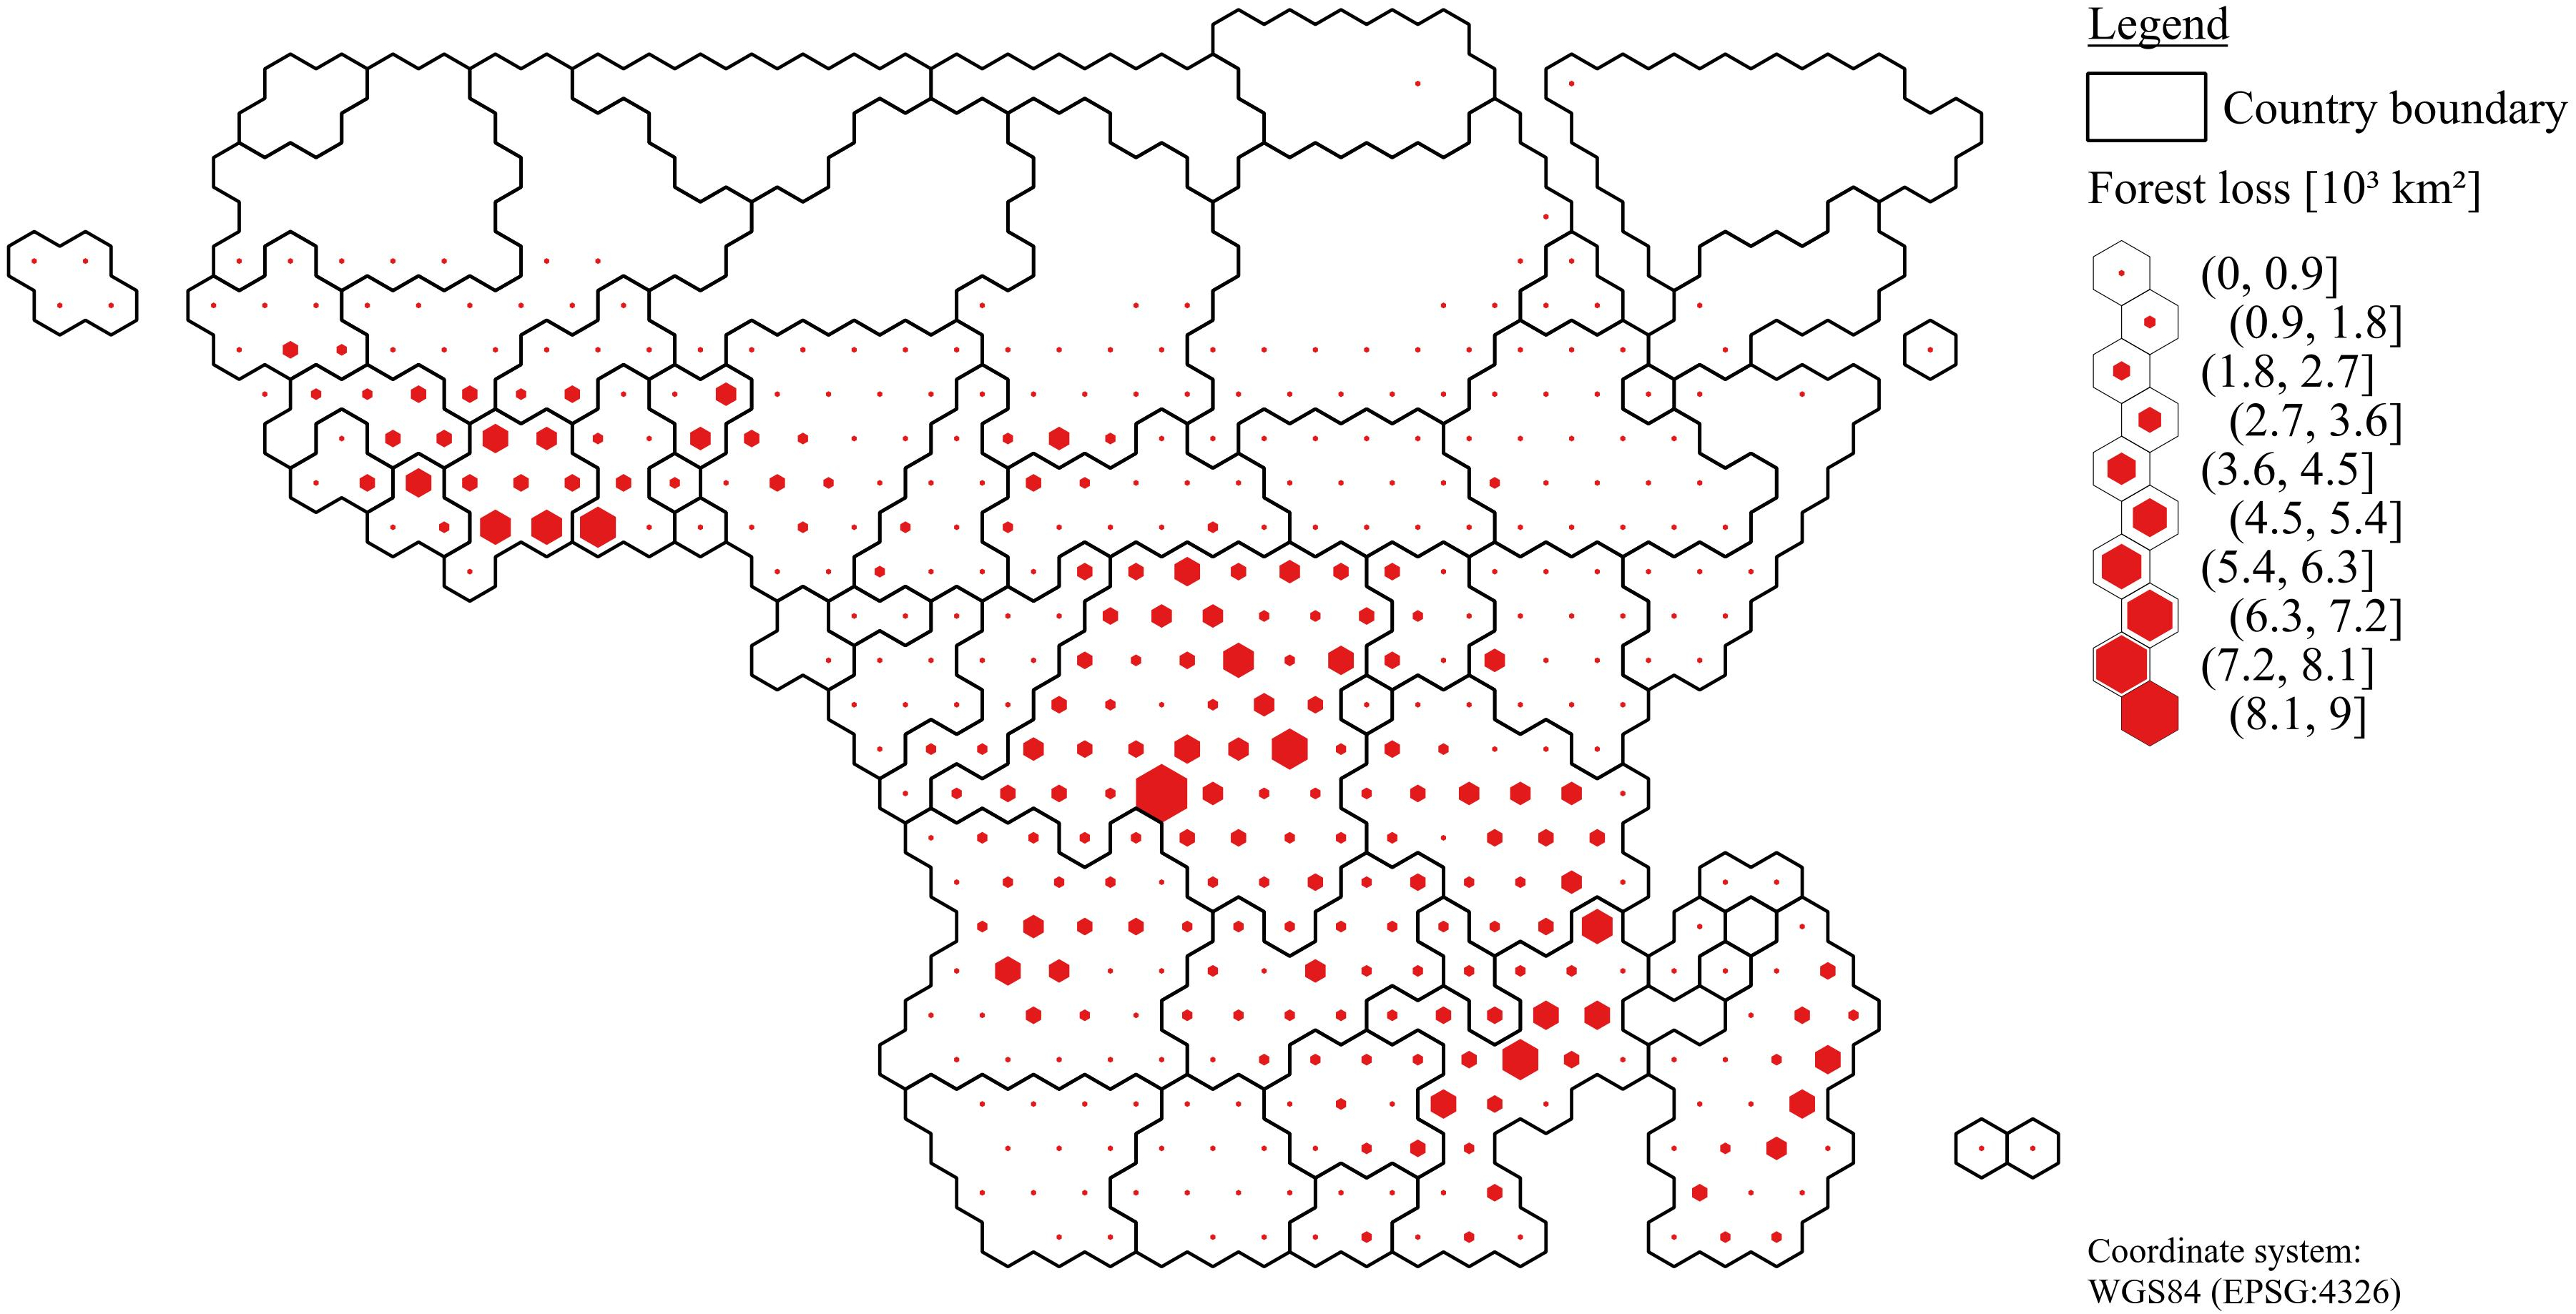
\includegraphics[scale=.9]{img/africa_loss_frameless}
				\caption[Tree cover loss in Africa between 2001 and 2010]{\textbf{Tree cover loss in Africa between 2001 and 2010:} This map shows the tree cover loss within our study extent between 2001 and 2010. An unscaled hexagon covers an area of 0.5 decimal degrees which translates to an area of approximately 49 thousand km$^2$ at the equator. Deforestation hot-spots with tree cover loss about 1.1 thousand km$^2$ per hexagon are located in Ivory Coast, Democratic Republic of the Congo, Angola, Mozambique, Madagascar, and Tanzania.}
				\label{fig:africa_loss}
			\end{figure}

			%old intro 
			%This section is intended to present a comprehensive insight in the tropical tree cover distribution within our study extent at 2000 over the tree continental regions. Further, we highlight at which sites the tree cover loss peaked between 2001 and 2010. The tree cover maps are derived from the \ac{GFC} tree cover 2000 layer while we selected only pixels within our forest definition which refers to the canopy density interval $(10,100]$. For an appropriate visualization of multivariate spatial data on a large extent we selected our hexagonal binning approach. For the tree cover maps we computed the total area covered by trees within a polygon and divide by the total area of the hexagon to determine the scaling. Additionally we aggregate the canopy density within a hexagon by applying the arithmetic mean. To arrange the tree cover loss maps we used our \ac{PDD} products. We computed the loss area within each hexagon for the following \ac{PDD} classes: cultivated land (10), regrowth (25), grassland (30), shrubland (40), artificial surfaces (80), and bareland (90). To determine the polygon scaling we divided the per hexagon loss area by the highest observed loss within a continental region. Forest cover, losses, and hexagon areas are computed by applying the Haversine equation. A hexagon in unscaled shape covers an area of 0.5 decimal degrees. The maps in this section should be interpreted as precursor to our \ac{PDD} predictions to detect regional and continental patterns of deforestation and as an example how large multivariate spatial data can be visualized and evaluated by a more advanced aggregation approach.

		\subsection{Mapping of proximate deforestation drivers}
		\label{subsec:results_proxy_deforestation_drivers}
			On the global scale the major \acp{PDD} are cropland and pastures which account for 20.2\% (177038.5 km$^2$) and 33.1\% (289445.5 km$^2$) as the table \ref{tab:proximate_driver} in the appendix \ref{ch:appendix_c} suggests. Regrowth dynamics account for 26.4\% (230 543.7 km$^2$) of the tree cover loss, while these dynamics include forestry activities, establishment of plantations, and plantation management practices like rotational cycle. The expansion of artificial surfaces account for 0.4\% (3690.1 km$^2$) of the forest loss, while the inundation of forests by rivers and lakes account for 1.4\% (12011.9 km$^2$). 

			In Latin America the transition of tree cover to cropland and pastures account for 21.3\% (95929.6 km$^2$) and 40.8\% (183841.4 km$^2$) as the table \ref{tab:proximate_driver} in the appendix \ref{ch:appendix_c} shows. Therefore, approximately 62\% (279771 km$^2$) of the tree cover were cleared for agricultural purposes in Latin America. Around 12.6\% (56909.3 km$^2$) of the tree cover loss is followed by tree cover regrowth, while the transition to shrubland account for 11.1\% (50260.2 km$^2$) of the tree cover loss, respectively. Minor \acp{PDD} are water, artificial surfaces, and bareland which account for 1.6\% (7169.9 km$^2$), 0.3\% (1561.5 km$^2$), and 0.1\% (405.4 km$^2$) of the forest transitions. \citet{Sy2015} estimates that agriculture accounts for 88.5\% of the tree cover loss, while transitions of forest cover to other \ac{LC} accounts for 11.5\%. Further, \citet{Hosonuma2012} achieve similar results for the conversion of tree cover to agricultural land where it accounts for approximately 90\% of the tree cover loss. Both studies estimate that the expansion of artificial surfaces account for approximately 1\% of the forest loss. The large difference could be explained by the definition of the forest transition classes in both studies. In both studies agriculture comprises pastures, cropland, and tree plantations. Additionally, both studies refer to the change of \ac{LU} and we determine the \acp{PDD} by the change of \ac{LC}. Further, \citeauthor{Sy2015} uses a sample based approach on 10x10 km \ac{FAO} FRA-2010 RSS data which could yield overestimates, while \citeauthor{Hosonuma2012} uses an empirical approach based on \ac{FAO} data as well. A recent study on \acp{PDD} estimates that commodity-driven deforestation, shifting agriculture, forestry, wildfire, and urbanization account for 56\%, 31\%, 13\%, 1\%, and <1\% of the tee cover loss, respectively \citep{Curtis2018}. Commodity-driven deforestation refers to tree cover loss as long-term permanent transition of forest to a non-forest \ac{LU} like agriculture which includes cropland, pastures, plantations and so forth. Comparable to the previously mentioned research on \acp{PDD} the difference between our estimates and \citeauthor{Curtis2018} arise from class definitions. If we would aggregate our \ac{LC} classes to their schema it would yield nearly the same results. In particular the same estimate for tree cover loss by urbanization shows that the similar classes without aggregation yield similar results. In Latin America the \ac{LC} change to cropland is mainly distributed over southern part, while the transition to pastures is concentrated in the central part of the continent as figure \ref{fig:americas_driver} suggests. Cropland expansion mainly took place in the south of Brazil, Paraguay, Argentina, and Bolivia, while forest loss by pasture expansion is concentrated in the center and north of Brazil. The spatial distribution of cropland/pasture dynamics largely corresponds to the findings of \citet{Graesser2015}. Large quantities of tree cover regrowth can be observed in the south-east and center of Latin America namely the southeast coast of Brazil and within the tropical rain forest covering Brazil, Peru, and Colombia. In south-east Brazil the findings of \citeauthor{Curtis2018} suggests that the regrowth dynamics are driven by forestry actions, while the coastline is exposed to shifting agriculture. Cropland and pasture expansion account for 19.1\% and 49.7\% of the tree cover loss, while regrowth dynamics and artificial surfaces account for 11.8\% and 0.3\% of the tree cover loss in Brazil. Figure \ref{fig:americas_driver} shows that deforestation by cropland expansion is mainly concentrated in the southern part of Brazil in the provinces Mato Grosso, Goi\'{a}s, and Mato Grosso do Sul, which is largely confirmed by \citet{Zalles2018} and \citet{Graesser2015}. Additionally, in the northern part of Mato Grosso and the southern part of Mato Grosso do Sul deforestation by grassland expansion can be observed \citep{Graesser2015,Sy2015}. The tree cover loss in the arc of deforestation can be attributed to pasture expansion, which is confirmed by \citet{Sy2015} and \citet{Graesser2015}. For the Chaco region of Paraguay the main \ac{PDD} is the expansion of cropland, which accounts for 48.9\% of the tree cover loss. The findings of \citet{Graesser2015} and \citet{Caldas2013} suggest that the main \ac{PDD} in this region is the expansion of pastures, while findings by \citet{Graesser2018} suggests that pastures are largely replaced by cropland \ac{LU} between 1990 and 2015. Therefore, the initial cause for tree cover loss could be the expansion of pastures but the \ac{LU} changed already to cropland at our image date of 2010. In the Argentinian part of the Chaco cultivated and grassland account for 65.8\% and 5.3\% of the tree cover loss. This could also be observed by \citet{Sy2015}. In Bolivia cropland and pasture expansion account for 37.2\% and 22.4\% of the forest loss, while transitions of forest cover to artificial surfaces account for 0.4\% of the tree cover loss, respectively. Main \ac{PDD} for the deforestation hot-spot in the province Santa Cruz is the expansion of cropland as figure \ref{fig:americas_driver} suggests. Further, in north Bolivia and at the Brazilian border the deforestation is driven by pasture expansion. Both patterns are largely confirmed by \citet{Graesser2015} and \citet{Sy2015}. In Guatemala cropland, pasture, and artificial expansion account for 23.9\%, 38.6\%, 0.5\% of the forest loss, respectively. The main \acp{PDD} for the deforestation hot-spot in the province of Peten are pasture expansion followed by cropland expansion as the map \ref{fig:americas_driver} suggests. Pasture expansion is the main force for deforestation in south of Guatemala. Regrowth dynamics in Guatemala which account for 12\% of the forest loss could be attributed to the establishment of oil palm plantations and shifting agriculture \citep{Furumo2017,Curtis2018}. In Peru cropland, pasture, and artificial expansion account for 6.6\%, 23\%, and 0.2\% of the forest loss, while regrowth dynamics account for 28.2\% of the forest loss, respectively. For the deforestation hot-spots located in the provinces of Huánuco, San Martin, and Ucayali the major \acp{PDD} are the expansion of pastures and regrowth dynamics. \citep{Sy2015} findings suggests that the expansion of cropland is the main deforestation driver in this central region of Peru. Regrowth dynamics in this region could be related to deforestation for oil palm plantations as the findings of \citet{Vijay2018} and \citet{Furumo2017} suggest. \citeauthor{Vijay2018} estimates that an area of approximately 845 km$^2$ is cleared for oil palm plantations between 2007 till 2013, while \citeauthor{Furumo2017} states that approximately an area of 156 km$^2$ forest is cleared for palm oil plantations between 2001 and 2014. Cultivated land, grassland, and regrowth dynamics account for 6.2\%, 33.4\%, and 24.7\% of the tree cover loss in Colombia, respectively. For the Colombian deforestation hot-spot located in the province of Cacquetá the expansion of pastures is the main \ac{PDD}, which is confirmed by \citet{Graesser2015}. This is also the case for the deforestation hot-spots located in the provinces of Bolívar and Antioquia.
			\begin{figure}[ht]
				\centering
				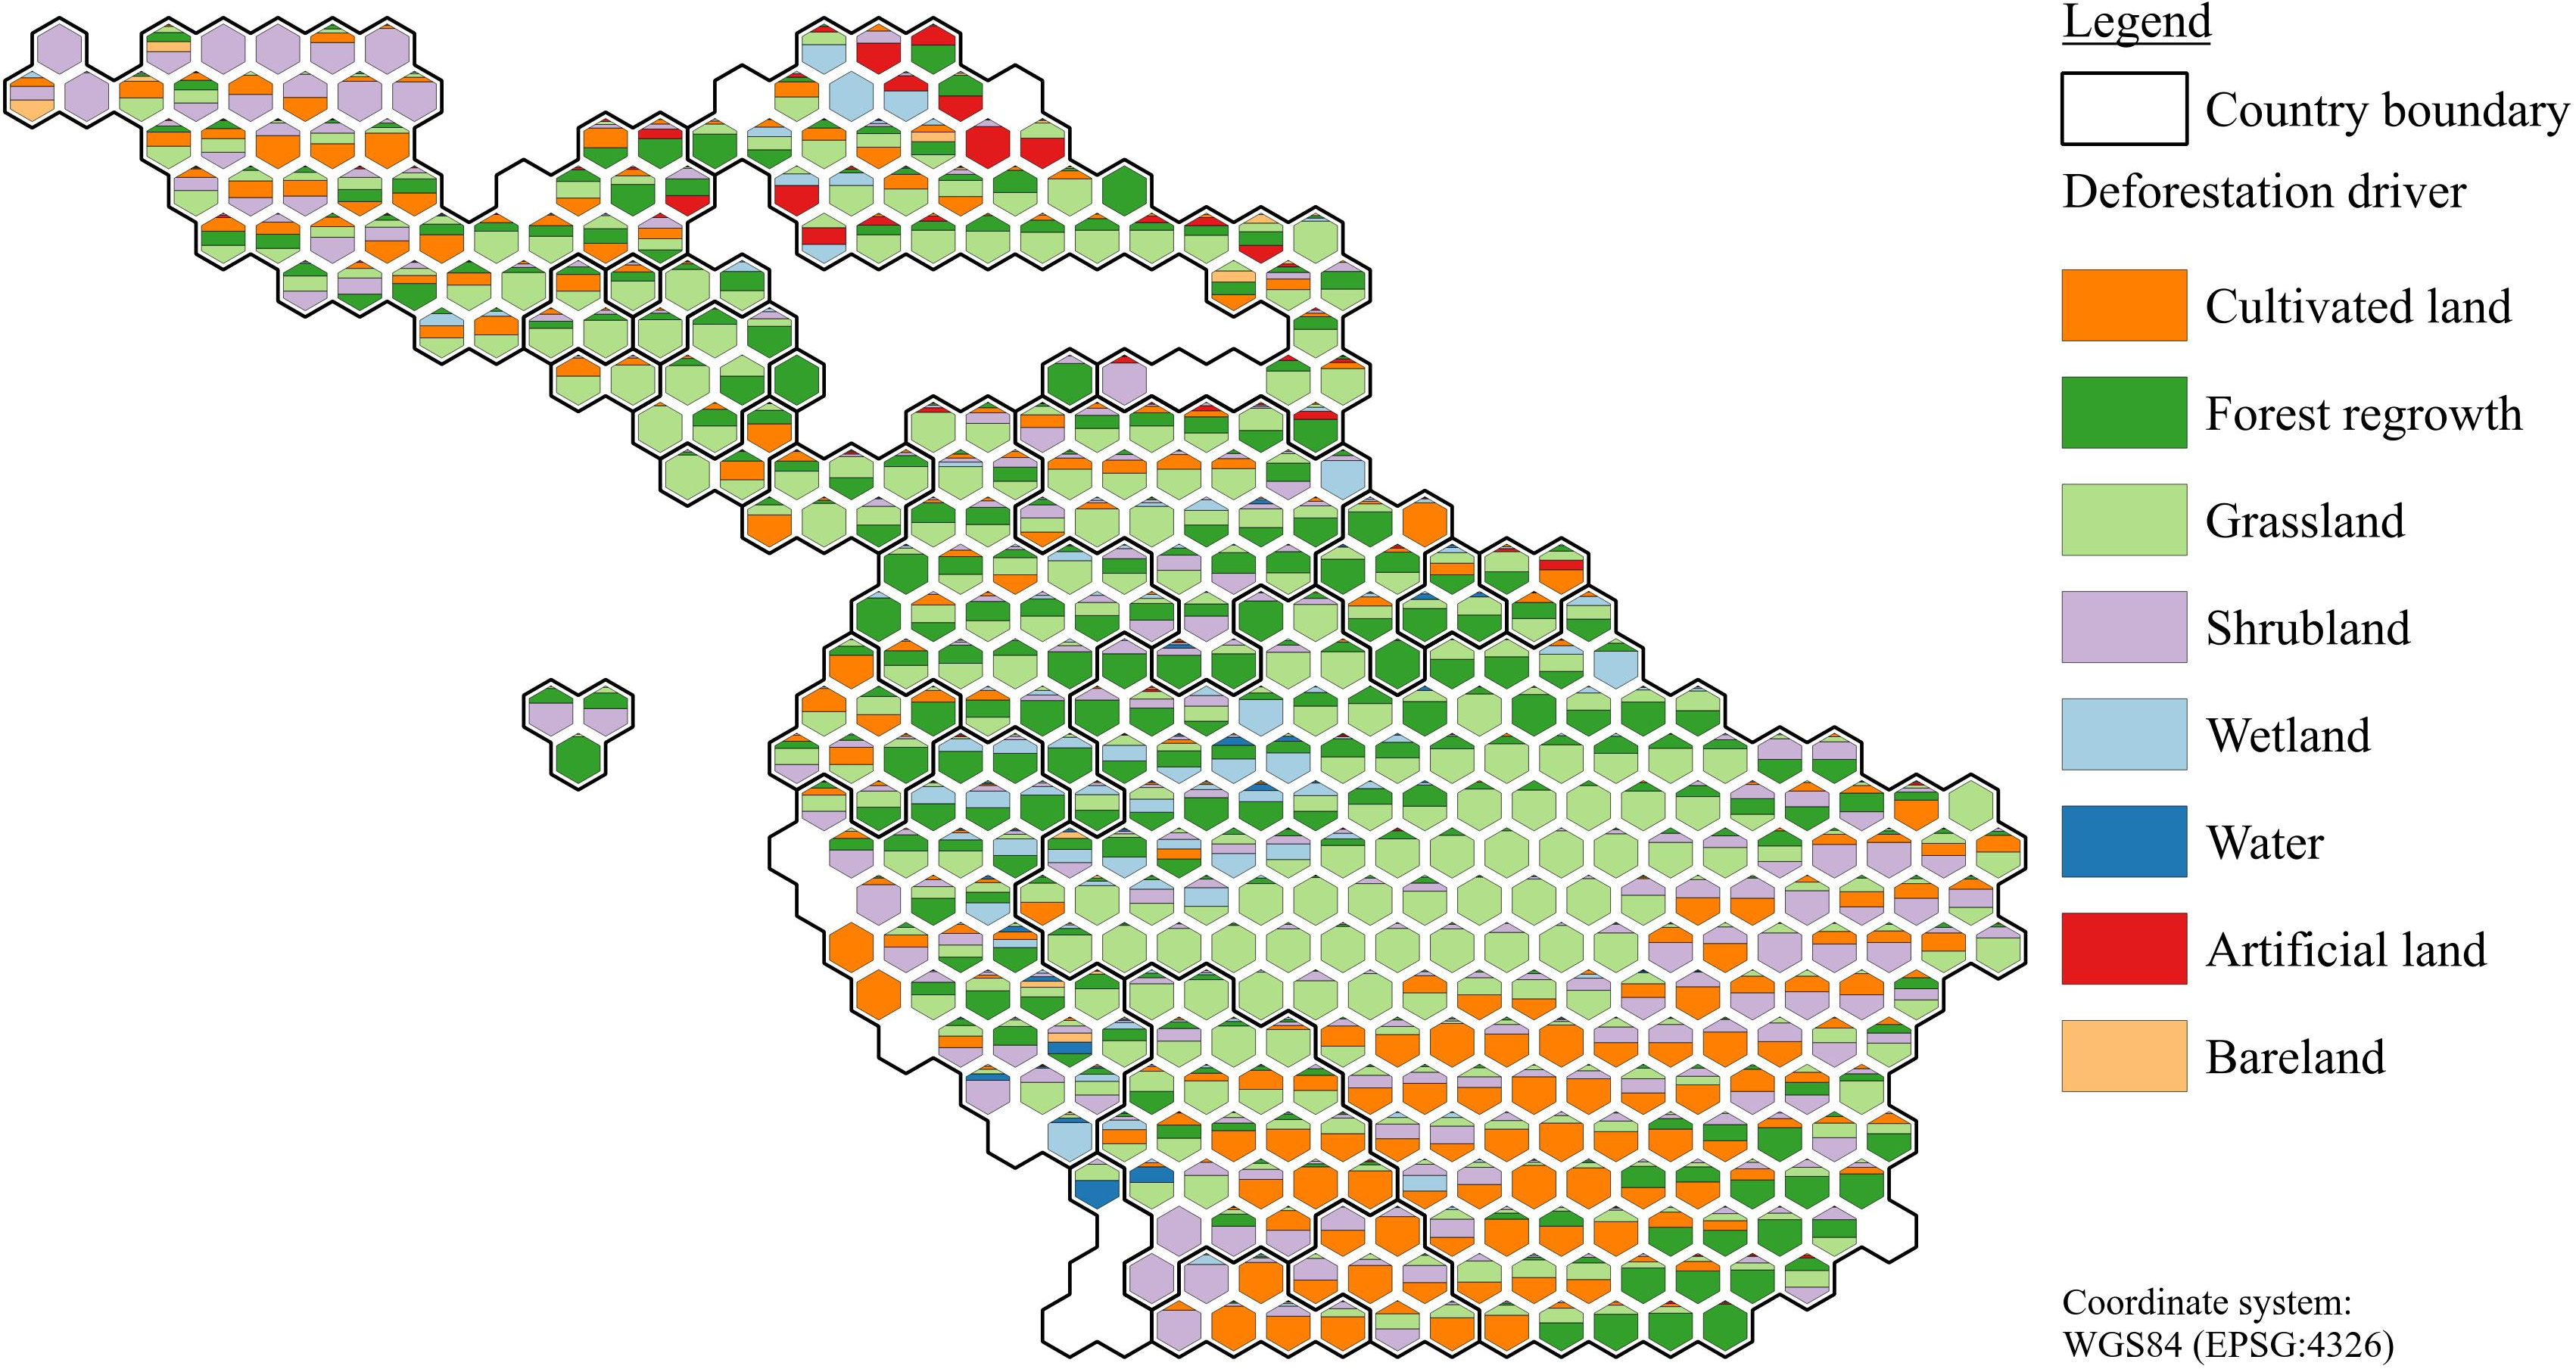
\includegraphics[scale=1]{img/americas_driver_frameless}
				\caption[Map of proximate deforestation drivers in Latin America]{\textbf{Map of proximate deforestation drivers in Latin America:} The map shows the distribution of proximate deforestation drivers in Latin America. The different sized and colored quantities within each hexagons interior shows the relative tree cover loss by a proximate deforestation driver. Scaling of a the hexagons is only intended for improving visual appeal.}
				\label{fig:americas_driver}
			\end{figure}

			For Asia/Australia the table \ref{tab:proximate_driver} in the appendix \ref{ch:appendix_c} shows cultivated and grassland account for 16\% (36819.3 km$^2$) and 7.1\% (16302.6 km$^2$) of the tree cover loss, respectively. Therefore, the transition of \ac{LC} to agriculture usage accounts for 23.1\% (53121.9 km$^2$) of the tree cover losses. The transition of tree cover to artificial surfaces and the forest loss by inundation by lakes and rivers account for 1.1\% (2431.9 km$^2$) and 0.4\% (890 km$^2$), respectively. In Asia/Australia the largest \ac{PDD} is the regrowth which accounts for 61.2\% (140653.4 km$^2$) of the cumulative tree cover loss. Forest transitions to shrubland account for 6.7 \% (), respectively. \citet{Hosonuma2012} estimates that \ac{LC} transitions by agriculture account for approximately 70\% of the forest loss, while \citet{Curtis2018} estimates that commodity-driven deforestation, shifting agriculture, forestry, wildfire, and urbanization account for 13\%, 78\%, 9\%, 13\%, <1\%, and <1\% of the tree cover loss in Southeast Asia, respectively. As mentioned in the previous paragraph the differences in \acp{PDD} estimates relate mainly to the applied methodology and the aggregation of \ac{LC} classes. The figure \ref{fig:asia_driver} shows an overview of the \acp{PDD} distribution in Asia/Australia and indicates that regrowth dynamics are largely concentrated at the east of Asia/Australia namely in the following countries: Indonesia, Malaysia, Philippines, and Papua New Guinea. Conversion of tree cover to cropland can be observed in Vietnam, Cambodia, the north of Thailand, and India in its entire extent. \citeauthor{Curtis2018} predicts that in Indonesia and Malaysia tree cover loss is largely driven by commodity-driven deforestation, while in Vietnam and Cambodia the forest loss is driven by commodity-driven deforestation and forestry. In Indonesia cropland and pasture expansion accounts for 15.4\% and 4.6\% of the forest cover loss, while regrowth dynamics account for the largest share of forest loss with 68.6\%. For the deforestation hot-spots concentrated on the Indonesian islands of Sumatra and Borneo (Kalimantan) the major \ac{PDD} are regrowth dynamics. This \ac{LC} transitions could be attributed to forest clearings for oil palm plantations and the rotational cycle of matured plantations which are commonly cleared after 18 years \citep{Corley2016}. \citeauthor{Corley2016} estimates that by 2010 an area of approximately 81 thousand km$^2$ is covered by palm oil plantations. \citet{Austin2019} estimates that forestry activities and oil palm plantations account 67\% of the tree cover loss, while agricultural expansion account for 35\% of the forest transitions in Indonesia between 2001 and 2015. For the islands of Sumatra and Borneo (Kalimantan) \citeauthor{Austin2019} predicts that more than a half of deforestation could be attributed to forestry and oil palm plantations. In Malaysia comparable to Indonesia regrowth dynamics account for the largest share of forest loss with 79.4\%. Cropland and grassland expansion account for 7.5\% and 2.6\% of the tree cover loss, respectively. The deforestation hot-spots are largely dominated by regrowth dynamics, which could be attributed to palm oil plantations and the related management practices like establishment of new sites and clearing of matured plantations. Whereas, the establishment of new sites is unlikely because the Malaysian industry has difficulties in finding appropriate sites for further expansion \citep{Corley2016}. \citeauthor{Corley2016} reports that by 2015 an area of approximately 50 thousand km$^2$ is covered by palm oil plantations. In Vietnam the \acp{PDD} cropland and pastures account for 32.8\% and 18.3\% of the tree cover loss, respectively. Further, regrowth dynamics account for 30.8\% of the tree cover loss. The deforestation hot-spots concentrated in the highlands are dominated by transitions to cropland, while the remaining part of the country is dominated by regrowth dynamics. The regrowth could be related to an increased reforestation effort, which is proved by expansion of natural forest cover \citep{Chazdon2008}. \citet{Curtis2018} predicts for the highland region that tree cover loss mainly can be attributed to commodity-driven deforestation. Cropland and pasture expansion account for 14.8\% and 16.4\% of the tree cover loss, while regrowth dynamics account for 57\% of the forest loss in Laos. The north and south of the country are dominated by regrowth dynamics, while expansion of cropland as second largest cause for deforestation. \citet{Curtis2018} data shows that the north is dominated by forestry activities and the south by commodity-driven deforestation.
			\begin{figure}[ht]
				\centering
				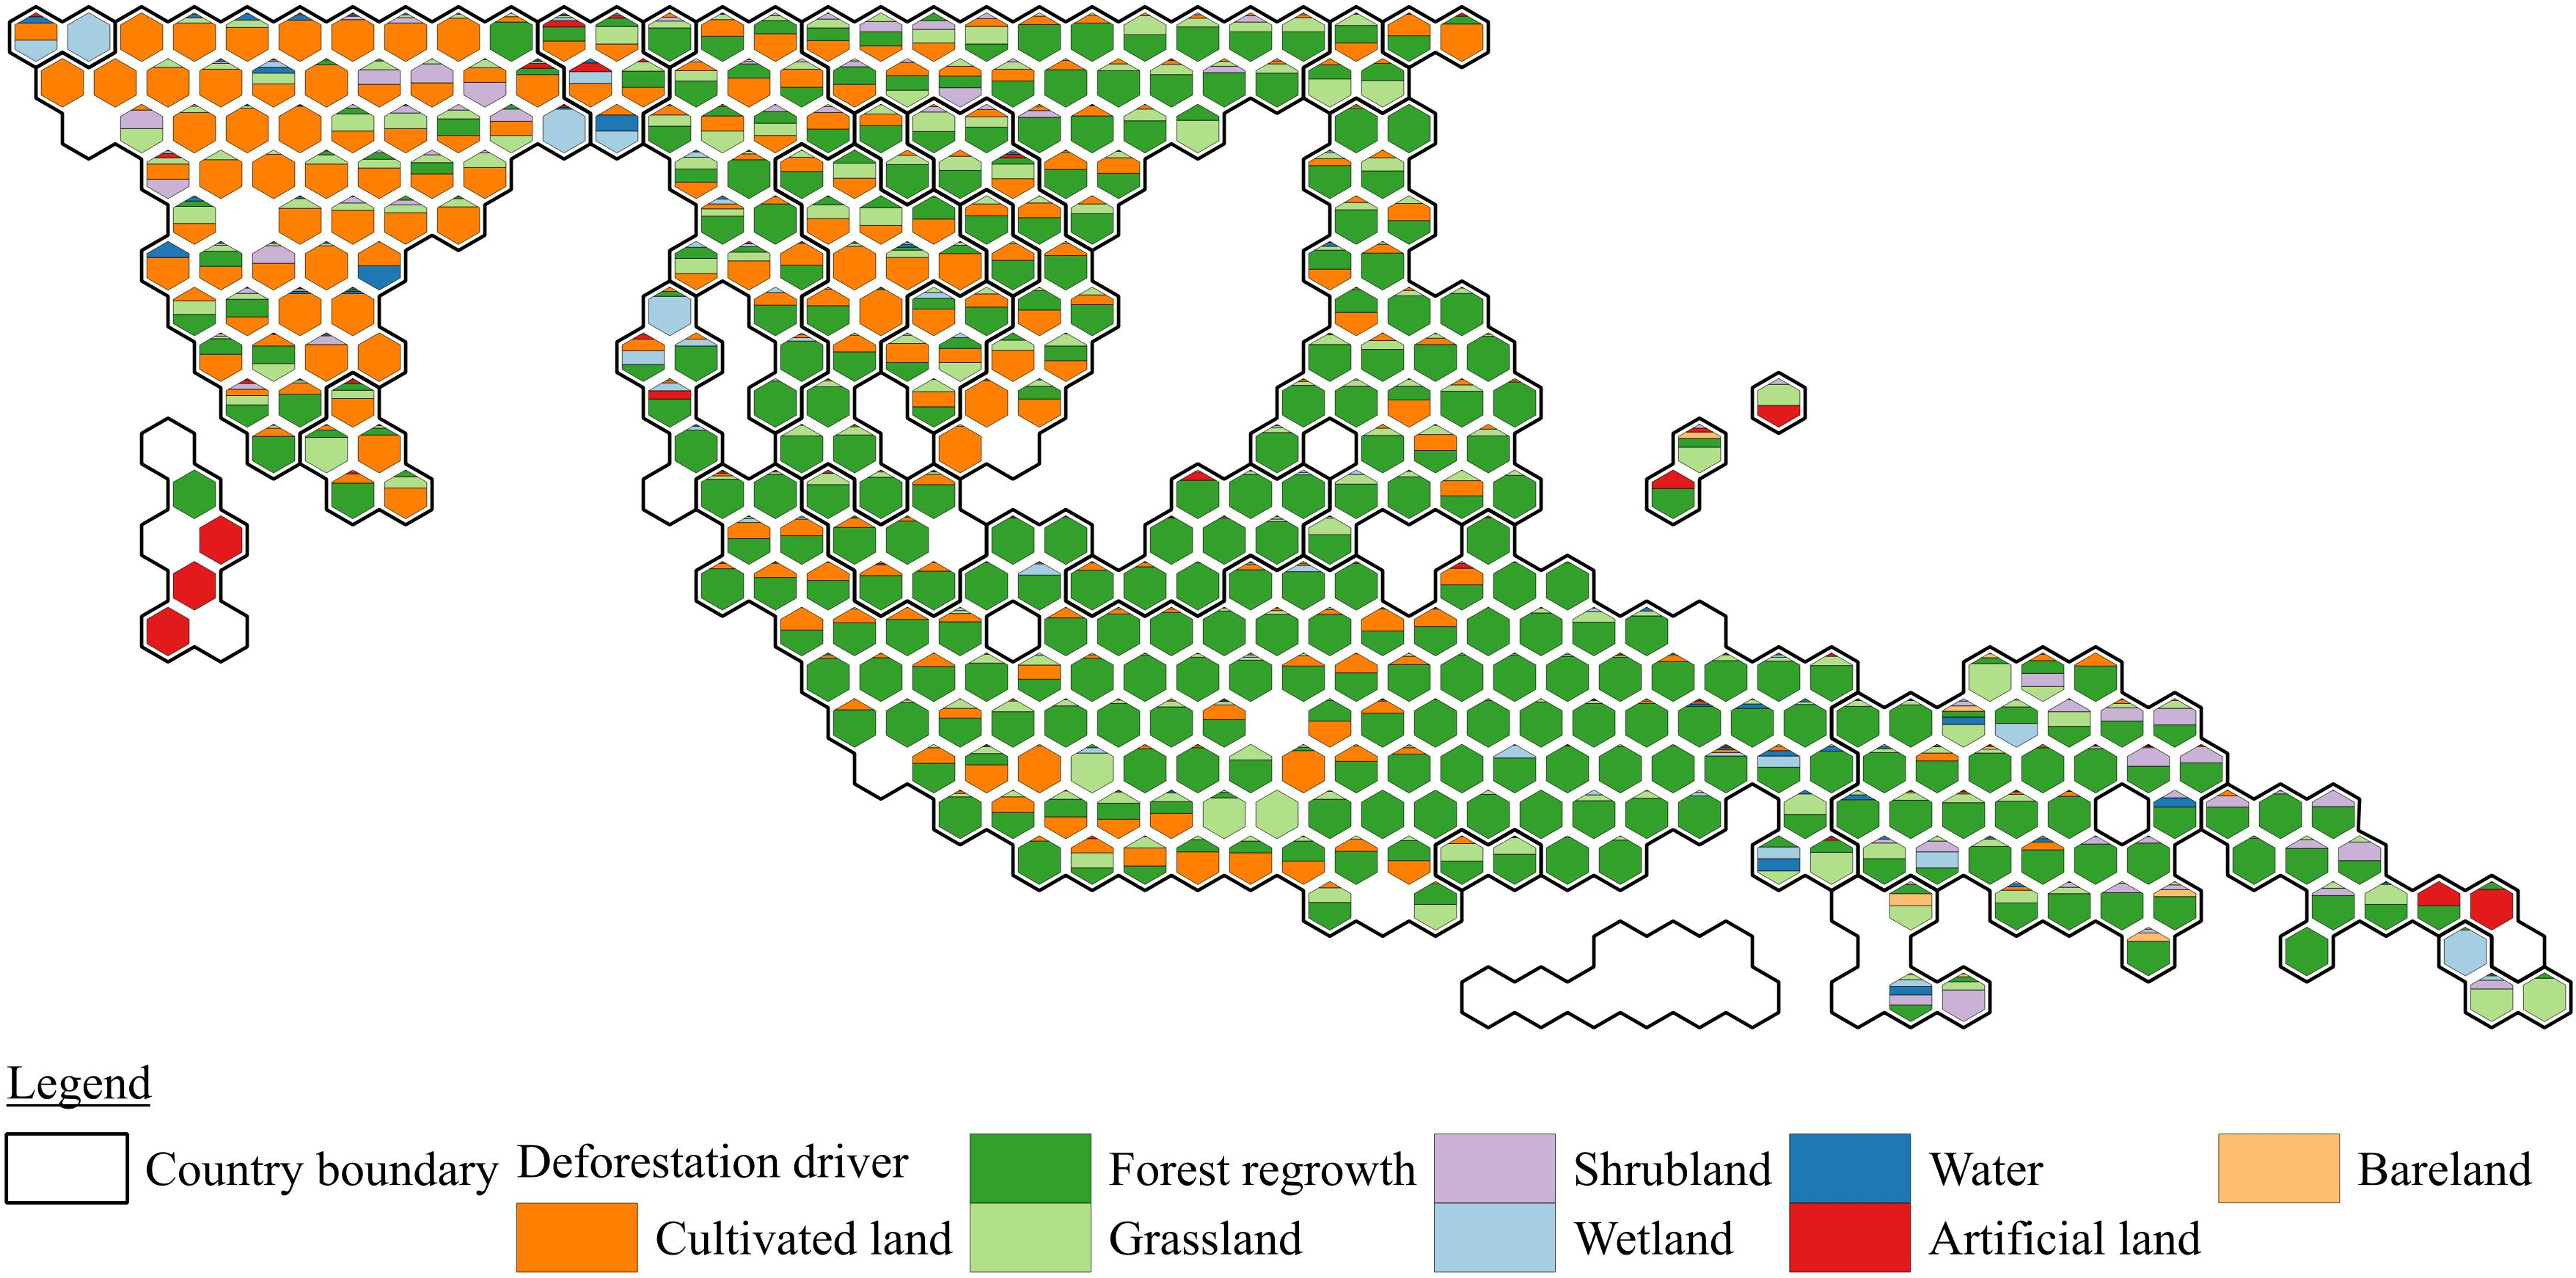
\includegraphics[scale=1]{img/asia_driver_frameless}
				\caption[Map of proximate deforestation drivers in Asia/Australia]{\textbf{Map of proximate deforestation drivers in Asia/Australia:} The map shows the distribution of proximate deforestation drivers in Asia/Australia. The different sized and colored quantities within each hexagons interior shows the relative tree cover loss by a proximate deforestation driver. Scaling of a the hexagons is only intended for improving visual appeal.}
				\label{fig:asia_driver}
			\end{figure}

			In Africa the table \ref{tab:proximate_driver} in the appendix \ref{ch:appendix_c} suggests that cropland and grassland account for 22.8\% (44289.5 km$^2$) and 46\% (89301.4 km$^2$) of the tree cover loss, respectively. Therefore, transitions to agricultural land are the major \ac{PDD} in Africa and account for 68.8\% (133590.9 km$^2$) of the tree cover loss. Forest transitions to water, artificial surfaces, and bareland account for 1.2\% (2409.9 km$^2$), 0.6\% (1238.6 km$^2$), and 0.1\% (146 km$^2$) of the tree cover loss, respectively. In Africa on 17\% (32980.8 km$^2$) of the area exposed to tree cover loss regrowth could be detected, while the transition to shrubland account for 3.4\% (6599.5 km$^2$) of the tree cover loss, respectively. The study on \acp{PDD} by \citet{Hosonuma2012} estimates that agriculture and urbanization account for approximately 75\% and 2\% of the tree cover loss, respectively. For Africa \citet{Curtis2018} shows that commodity-driven deforestation, shifting agriculture, forestry, wildfire, and urbanization account for 4\%, 92\%, 4\%, <1\%, <1\% of the tree cover loss. The figure \ref{fig:africa_driver} shows the distribution of \acp{PDD} in Africa and indicates that the forest loss in the east of the continent is largely driven by the expansion of cultivated land. This can be observed in the following east African countries: Tanzania, Mozambique, Zambia, Malawi, and Zimbabwe. The central African countries like Democratic Republic of the Congo, Central African Republic, Congo, and South Sudan are mainly exposed to expansion of pastures as the map suggest. The findings of \citeauthor{Curtis2018} suggest that overall countries in Africa the major deforestation driver is shifting agriculture. At the Ivory coast cropland and pasture expansion account for 12.5\% and 46.9\% of the forest loss, respectively. The figure \ref{fig:africa_driver} shows that the north of the country is dominated by grassland and cropland transitions, while the south is dominated by pasture and regrowth tree cover transitions. To best of our knowledge no study except \citeauthor{Curtis2018} tried to estimate the general spatial distribution of \acp{PDD} at the Ivory Coast. However, there are studies that investigate the expansion of cocoa farmings as one of the major deforestation drivers in this country \citep{Barima2016,Ruf2014}. Both studies mention that cocoa farming shifted to the south-west of the country where a large quantities of regrowth are observable on figure \ref{fig:africa_driver}. Cocoa plantations are tree crops therefore they must appear as regrowth signal. \citet{Curtis2018} predicts that in the south-western part of the country deforestation are mainly driven by shifting agriculture. The expansion of cropland and pastures account for 9.4\% and 52\% of the forest loss, while regrowth dynamics account for 26.6\% of the tree cover loss in the Democratic Republic of the Congo. For the deforestation hot-spot around the Congo river the major \ac{PDD} is the expansion of grassland, while the northern hot-spots are dominated by grassland and regrowth transitions. \citet{Ickowitz2015} mention in his comprehensive literature review on agriculture and deforestation in the Democratic Republic of the Congo that the major deforestation driver is shifting agriculture. Therefore grassland transition can be fallow land which is later transformed to the regrowth class by natural regeneration. Further, \citeauthor{Curtis2018} observed in his study that shifting agriculture is the main deforestation driver. In Angola cultivated and grassland account for 32.7\% and 54.7\% of the deforestation, respectively. The deforestation hot-spots in Angola are mainly dominated by pasture and cropland expansion, which is also observable for the rest of the country. \citet{Cabral2011} performed a case study on deforestation in the province of Huambo that show evidences that cropland area increased between 1990 and 2009. To best of our knowledge only \citet{Curtis2018} performed a spatial explicit study on deforestation driver which includes entire Angola. This study shows that tree cover loss can be attributed to shifting agriculture as the rest of Africa. Cropland and pasture expansion account for 32.7\% and 45.6\% of the tree cover loss, respectively. The northern part of the country is dominated cropland and regrowth expansion dynamics, while for the deforestation hot-spots located in the provinces of Zambezia and Nampula the major \acp{PDD} are cropland, pasture, and regrowth expansion. A literature review performed by \citet{Sitoe2012} reveals that deforestation is a multi-phase process, where hardwood extraction and firewood collection is followed by steady conversion of forest to agricultural \ac{LC}. Further the total area occupied by cropland increased by 59\% from 2001 to 2010. In Madagascar regrowth dynamics account for 40.6\% of the tree cover loss, while grassland account for 44.6\% of forest loss. The north-east coast of Madagascar is dominated by pasture expansion and regrowth dynamics. \citet{Curtis2018} predicts that the major \ac{PDD} is shifting agriculture other studies on the distribution of \acp{PDD} are only as small scale case studies available. Largest deforestation driver in Tanzania are cropland and pastures, which account for 42.1\% and 40.6\% of the tree cover loss. The deforestation hot-spots are mainly exposed to cropland and grassland expansion, while in the north-west-center of the country the major \ac{PDD} is cropland and in the south-east is grassland. To best of our knowledge no study estimate spatial explicit the \acp{PDD} of tree cover loss for Tanzania except the study of \citet{Curtis2018}, which predicts that the major driver is shifting agriculture. A case study on forest loss in the province of Kilwa shows evidences that the total cropland area increased by 40\% from 2005 to 2010.
			\begin{figure}[ht]
				\centering
				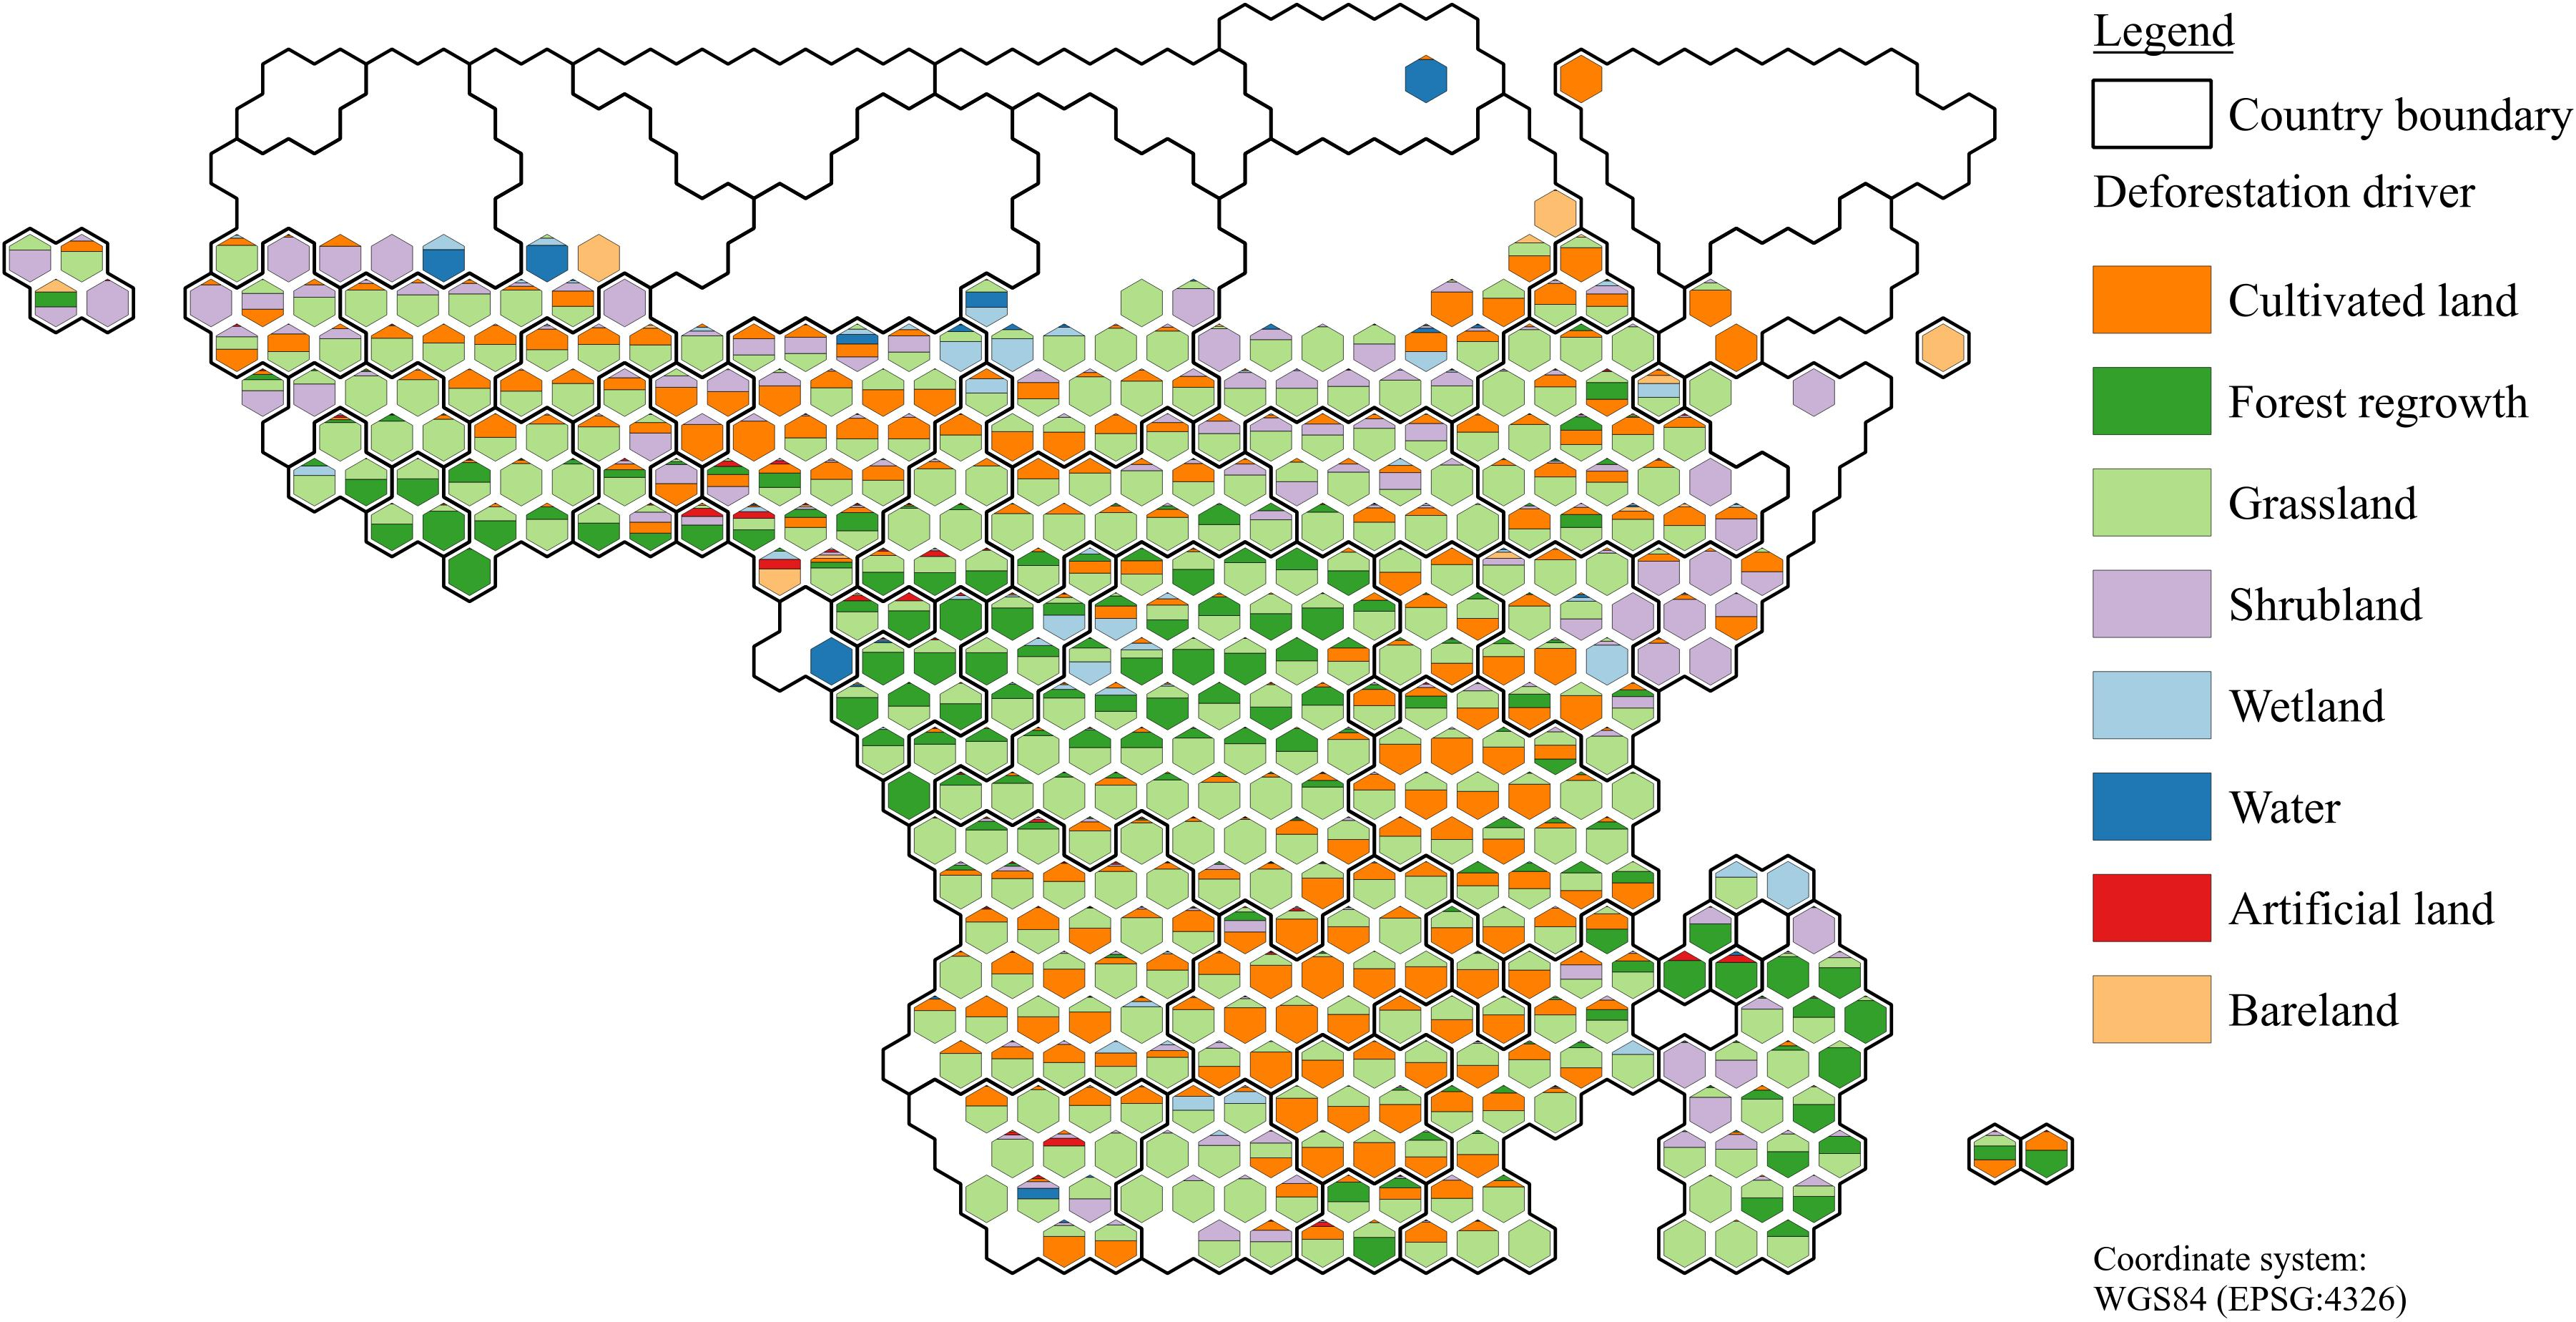
\includegraphics[scale=1]{img/africa_driver_frameless}
				\caption[Map of proximate deforestion drivers in Africa]{\textbf{Map of proximate deforestation drivers in Africa:} The map shows the distribution of proximate deforestation drivers in Africa. The different sized and colored quantities within each hexagons interior shows the relative tree cover loss by a proximate deforestation driver. Scaling of a the hexagons is only intended for improving visual appeal.}
				\label{fig:africa_driver}
			\end{figure}

			%old intro
			%Our goal is to estimate the distribution of \acp{PDD} over the tropical zone, the continental range, and at a country scale for the time frame of 2001 till 2010. We achieved this estimate by superimposing the annual tree cover losses and aggregated gains of the \ac{GFC} datasets and the \ac{GL30} land cover map from 2000. We carefully selected our global definition of tree cover in the canopy density interval $(10,100]$ by applying the Jaccard Index and statistical testing detailed in section \ref{subsec:results_forest_definition}. By using this canopy density interval we filtered the \ac{GFC} annual losses and we considered tree cover gains only within previously lost tree cover. After superimposing we applied a reclassification of tree cover losses still classified as forest by the \ac{GL30} layer. We aggregated this structures by clustering and applied a square sized buffer of 500 meter side length. Next, we reclassified the structure by determining the highest frequent \ac{LC} class within the buffer. For further details on the \ac{PDD} prediction refer to section \ref{subsubsec:methods_proximate_deforestation_driver}. The \ac{PDD} distribution choropleth-maps for Latin America, Asia/Australia, and Africa we derived by applying our hexagonal-binning approach in combination with a hexagon-pie-chart. A hexagon in unscaled shape covers an area of 0.5 decimal degrees. Section \ref{subsec:methods_binning} describes detailed how we derived these cartograms. 

		\subsection{Accuracy assessment}
		\label{subsec:results_accuracy_assessment}
			This section presents and discuses the accuracy assessment of the \acp{PDD} prediction layer, while the table \ref{tab:results_confusion_matrix} shows the results of this assessment. We performed an accuracy assessment for 6000 randomly drawn samples over the entire study scale. We stratified our study region by continents and selected 10 sampling tiles per strata. From each tile we selected by random 200 \ac{LC} transition locations. By using high resolution imagery from Google Maps/Earth we created a set of ground-truth labels, which refers to the reference section in table \ref{tab:results_confusion_matrix}. From the 6000 samples cultivated land (10), forest (20), regrowth (25), grassland (30), shrubland (40), wetland (50), water (60), artificial surfaces (80) and bareland (90) account for 14.5\%, 18.2\%, 26.8\%, 30.5\%, 7.3\%, 1.2\%, 0.5\%, 0.8\%, and 0.1\% of the samples, respectively. This corresponds to the relative distribution of the  \acp{PDD} in table \ref{tab:proximate_driver} in the appendix \ref{ch:appendix_c}. In total 4560 of 6000 \ac{LC} transitions are correctly classified by our approach to predict \acp{PDD} of tropical deforestation. This translates to an overall accuracy of approximately 0.76, which implies that approximately 76\% of the forest loss is correctly classified. For the classification of tree cover losses as cultivated land the producers and users accuracy account for 0.85 and 0.84, respectively. Therefore, this class is achieve the highest certainty and a tendency to overestimation or underestimation is not give. For the regrowth class producers and users accuracy account for 0.88 and 0.72, respectively. This shows that regrowth is slightly overestimated, while this class was introduced by the \ac{GFC} gain layer. Section \ref{subsec:methods_gfc} explains that tree cover gains are underestimated but these underestimates are captured by the forest class. 
			For the grassland class producers and users accuracy account for 0.77 and 0.80, respectively. In general this class show no tendencies of over- or underestimates. The transformation of forests to artificial surfaces is largely underestimated as the difference of producers and users accuracy which account for 0.42 and 0.82 show. This could be attributed to our reclassification approach. Further, the bareland class is underestimated as well, which could be attributed to the reclassification approach. The wetland class achieves a accuracy of 0.51, while the users accuracy highlights that this class is underestimated. Wetlands are highly dynamic ecosystems therefore for this class it is to expect that the accuracy is lower. For water bodies the producers and users accuracy account for 0.67 and 0.68, which shows no general tendency of underestimation or overestimation. For the shrubland class the producers and users accuracy account for  .71 and .81, while this shows that this class is underestimated. As beforehand mentioned the reclassification approach could lead to this effect. The reclassification tends to favorite class with a higher probability. 
			\begin{table}[ht]
				\centering
				\caption[Accuracy assessment]{\textbf{Accuracy assessment:} We selected 200 samples by random from 10 randomly selected tiles from the three sampling stratas Latin America, Asia/Australia and Africa. Labels refer to our proximate deforestation driver classes, which are detailed in section \ref{subsubsec:methods_proximate_deforestation_driver}. Reference refers to the samples we classified by visual interpretation of Google Maps high resolution imagery and predictions refer to the label the sample has in our proximate driver product. The abbreviations PAc, UAc, OvAc, Com, Om, Tot, and Kappa refer to the terms Producers-Accuracy, Users-Accuracy, Overall-Accuracy, Error of Commission, Error of Omission, row or column total, and Kappa Coefficient.}
				\label{tab:results_confusion_matrix}
				\begin{tabular}{llrrrrrrrrrrrr}
					\hline
					& & \multicolumn{9}{c}{Reference} & & & \\\cline{3-11}
					& Cls & 10 & 20 & 25 & 30 & 40 & 50 & 60 & 80 & 90 & Tot & UAc & Om \\\hline
					\multirow{9}{*}{\STAB{\rotatebox[origin=c]{90}{Prediction}}}
					& 10 & 730 & 37 & 62 & 15 & 16 & 2 & 3 & 5 & 0 & 870 & .84 & .16 \\ 
					& 20 & 41 & 744 & 56 & 189 & 31 & 12 & 0 & 15 & 4 & 1092 & .68 & .32 \\ 
					& 25 & 29 & 202 & 1155 & 172 & 22 & 10 & 5 & 11 & 4 & 1610 & .72 & .28 \\ 
					& 30 & 36 & 187 & 32 & 1466 & 73 & 21 & 0 & 17 & 0 & 1832 & .80 & .20 \\ 
					& 40 & 14 & 21 & 4 & 41 & 352 & 1 & 1 & 2 & 1 & 437 & .81 & .19 \\ 
					& 50 & 0 & 5 & 3 & 10 & 4 & 50 & 0 & 1 & 0 & 73 & .68 & .32 \\ 
					& 60 & 2 & 1 & 0 & 3 & 0 & 2 & 18 & 2 & 0 & 28 & .64 & .36 \\ 
					& 80 & 3 & 3 & 0 & 1 & 1 & 1 & 0 & 40 & 0 & 49 & .82 & .18 \\ 
					& 90 & 0 & 0 & 0 & 1 & 0 & 0 & 0 & 3 & 5 & 9 & .56 & .44 \\\hline 
					& Tot & 855 & 1200 & 1312 & 1898 & 499 & 99 & 27 & 96 & 14 & 6000 & & \\
					& PAc & .85 & .62 & .88 & .77 & .71 & .51 & .67 & .42 & .36 & Kappa & \multicolumn{2}{r}{OvAc} \\
					& Com & .15 & .38 & .12 & .23 & .29 & .49 & .33 & .58 & .64 & .69 & \multicolumn{2}{r}{.76} \\ \hline
				\end{tabular}
			\end{table}

	\section{Carbon losses}
		On global scale the removal of \ac{AGB} account for a gross carbon loss of approximately 12964 MtC between 2001-2010 (table \ref{tab:soce_tab}). \citet{Achard2014} estimates that the gross carbon loss from tropical deforestation is between 6020-12370 MtC for the same period. The gross carbon loss by soil organic carbon change is between 478-688 MtC if we assume that all deforestation occurs within primary forest (SC$_1$). For the second scenario (SC$_2$) we estimated a carbon loss between 226-378 MtC. In Latin America the gross carbon loss account for approximately 6144 MtC for the removal of \ac{AGB} by tropical tree cover loss (table \ref{tab:soce_tab}). \citet{Achard2014} estimates that the gross carbon loss is between 3226-6497 MtC for the period 2001-2010, while \citet{Sy2015} measures a carbon loss in magnitude between 5959-6961 MtC between 1990-2005. The comparison with our estimates shows, that our results not largely differ from the literature although the methodology differs.
		For Asia/Australia the removal of \ac{AGB} accounts for a gross carbon loss of approximately 3955 Mt C (table \ref{tab:soce_tab}), while \citep{Achard2014} estimates a carbon loss between 2355-3670 MtC for the period 2001-2010.
		In Africa the gross carbon loss account for approximately 2865 MtC, while \citep{Achard2014} measures a carbon loss between 430-2220 MtC for the period 2001-2010.
		\begin{table}[ht]
			\centering
			\caption[Carbon losses]{\textbf{Carbon losses:} Carbon losses by the removal of aboveground woody biomass and soil organic carbon change. The columns SC$_1$ and SC$_2$ refer to the gross carbon loss by soil organic carbon change, while the column AGB refers to carbon loss by biomass removal. The unit of the values is MtC and standard errors are given in brackets.}
			\label{tab:soce_tab}
			\begin{tabular}{lrrrr}
				\hline
				Region & SC$_1$ & SC$_2$ && AGB\\\hline
				Latin America & 259 ($\pm$ 44) & 165 ($\pm$ 44) && 6144\\
				Asia/Australia & 220 ($\pm$ 43) & 76 ($\pm$ 16) && 3955\\
				Africa & 104 ($\pm$ 18) & 61 ($\pm$ 16) && 2865\\
				Global & 583 ($\pm$ 105) & 302 ($\pm$ 76) && 12964\\\hline
			\end{tabular}
		\end{table}

	\section{Ecosystem service values}
		Between 2001 and 2010 on a global scale tree cover loss of approximately 772 thousand km$^2$ accounts for a \ac{ESV} loss of 414.1, 405.2, and 101.1 billion dollar per year as table \ref{tab:esv_results} shows. By applying the \ac{ESV} coefficient for tropical forest from \citet{Costanza2014} the expansion of cropland and pastures account for a loss of approximately 95.3 and 128 billion dollar per year, respectively. The transition of forest cover to artificial surfaces and regrowth dynamics account for 2.3 and 124 billion dollar per year. If we consider the monetary value of tropical forest from \citet{Siikamaki2015} cropland, grassland, artificial surfaces, and regrowth dynamics account for a loss of approximately 23.2, 46.7, 0.5, and 30.2 billion dollar per year, respectively. The gross gain in \ac{ESV} from \ac{LC} transitions of tropical forest cover accounts for 350.6, 208.7, and 31.0 billion dollar per for the three datasets. By using the coefficients from the first dataset cropland, pastures, artificial surfaces, and regrowth dynamics account for a gain of 98.5, 120.6, 2.4, and 124.1 billion dollar per year, respectively. If we consider \citet{Groot2012} grassland and regrowth account for a gain of 83 and 121 billion dollar per year, while regrowth dynamics account for a gain of approximately 31 billion dollar for the last dataset. On global scale the net balance of tropical forest change account for -63.5, -196, and -70.1 billion dollar per year for the three datasets Co, Dg, and Wb, respectively. The greatest net loss can be observed by applying \citeauthor{Groot2012} \ac{ESV} coefficients which could be mainly attributed to the small number of \acp{PDD} classes which correspond to a evaluated \ac{ESV} biome. The relative small net loss in \ac{ESV} by using the coefficients from the first dataset is attributed on the fact that approximately a fifth of the global tree cover is lost by the expansion of cropland. \citeauthor{Costanza2014} estimates 5567 Int'I\$ y$^{-1}$ as the \ac{ESV} for cropland which is 1.03 times greater than the \ac{ESV} of tropical forest. Further, nearly a quarter of tropical forest cover is exposed to regrowth dynamics which uses the equivalent \ac{ESV} as tropical tree cover. Therefore, approximately a half of the tropical forest loss is replaced by \ac{LC} which has a greater or equal \ac{ESV} than the \ac{ESV} of tropical forest. For the time frame 2000 till 2012 \citet{Song2018} estimates that the net loss of tropical forest cover accounts for a \ac{ESV} loss of 550.7 billion dollar per year. The difference between our \ac{ESV} loss can be attributed to discrepancies in \ac{LC} change estimates, forest definition, and temporal resolution. \citeauthor{Song2018} considered the tree cover loss in all canopy densities and used for his net loss estimate tree cover gains within former forested area and the establishment of new tree cover. Further, \citet{Costanza2014} estimates that tropical forest loss account for a \ac{ESV} loss of 3.5 trillion dollar per year between 1997 and 2011. The large differences can be attributed to forest loss area estimates and the time scale of the study.
		\begin{table}[ht]
			\centering
			\caption[Ecosystem service value balance]{\textbf{Ecosystem service value balance:} The dataset column refers to the three global ecosystem service value datasets by \citet{Costanza2014} (Co), \citet{Groot2012} (Dg), and \citet{Siikamaki2015} (Wb). Loss refers to the monetary value of tropical forest deforested by the following aggregated anthropogenic proximate deforestation drivers: cropland, grassland, regrowth, shrubland, artificial surfaces, and bareland. Gain is the monetary value of the land cover transition and balance is difference of gain and loss. Monetary unit of the ecosystem service values is 10$^{9}$ 2007 Int'I\$ y$^{-1}$ (billion international dollar 2007 per year).}
			\label{tab:esv_results}
			\begin{tabular}{lrrrr}
				\hline
				Dataset & Latin America & Asia/Australia & Africa & Global\\
				\hline
				Co$_{loss}$ & 208.3 & 111.6 & 94.2 & 414.1 \\
				Co$_{gain}$ & 161.0 & 109.1 & 80.6 & 350.6 \\
				Co$_{balance}$ & -47.3 & -2.5 & -13.6 & -63.5\\
				Dg$_{loss}$ & 204.0 & 109.1 & 92.1 & 405.2\\
				Dg$_{gain}$ & 82.5 & 83.1 & 43.1 & 208.7\\
				Dg$_{balance}$ & -121.5 & -26.0 & -49.0 & -196.5\\
				Wb$_{loss}$ & 51.0 & 27.2 & 22.9 & 101.1\\
				Wb$_{gain}$ & 7.3 & 19.4 & 4.3 & 31.0 \\
				Wb$_{balance}$ & -43.7 & -7.8 & -18.6 & -70.1 \\
				\hline
			\end{tabular}
		\end{table}

		In Latin America a forest loss of approximately 396 thousand km$^2$ accounts for 208.3, 204, or 51 billion 2007 Int'I\$ y$^{-1}$ of \ac{ESV} loss as table \ref{tab:esv_results} suggests. By applying the \citet{Costanza2014} monetary value for tropical forest the transition of tree cover to cropland accounts for a loss of 51 billion Int'I\$ y$^{-1}$, while transitions to pastures account for a loss of approximately 126 billion dollar per year. The tropical deforestation by the expansion of artificial and bareland surfaces account for a loss of 1 billion Int'I\$ y$^{-1}$, while regrowth dynamics convert to a loss of 30 billion dollar. By using the monetary value of tropical forest from \citet{Siikamaki2015} the transitions to cropland and pastures cost 12.6 and 30.6 billion dollar, respectively. Further, the aggregated urbanization and bareland transition accounts for 0.3 billion dollar per year, while regrowth dynamics account for 7.5 billion international dollar per year. The variability in the estimates is related to the difference of monetary value for tropical forest between both datasets. \citeauthor{Costanza2014} monetary prediction for tropical forest is approximately 4 times greater than \citeauthor{Siikamaki2015}. We estimated a gross monetary gain of 161 billion dollar per year for the Co dataset. The table \ref{tab:esv_mapping} in section \ref{subsec:methods_esv} suggests that we calculated the monetary gain from \ac{LC} transitions to cropland, grassland, artificial surfaces, and regrowth which account for 53.4, 76.6, 1, and 30.6 billion dollar per year, respectively. By applying \citet{Groot2012} \ac{ESV} estimates the gross gain from \ac{LC} transitions account for 82.5 billion dollar per year. This converts to a monetary gain from grassland and regrowth transitions of approximately 52.8 and 29.9 billion dollar. The last dataset we tested enabled us to compute only the \ac{ESV} gain from tree cover regrowth which accounts for a monetary gain of 7.3 billion dollar per year, respectively. In Latin America the net balance of \ac{ESV} changes account for -47.3, -121.5, and -43.7 billion dollar for Co, Dg, and Wb, respectively. The negative signs indicates that overall three datasets the we could observe a net loss of \ac{ESV} in Latin America for the time period 2001 till 2010. The highest net loss can be observed for the Dg dataset but this relate to the small number of \ac{LC} transitions defined by a monetary value.

		For our study period in Asia/Australia tree cover loss of approximately 230 thousand km$^2$ accounts for an \ac{ESV} loss of 111.6, 109.1, or 27.2 billion dollar per year for the three datasets as table \ref{tab:esv_results} shows. The first dataset predicts that forest cover transitions to cultivated- and grassland account for a loss of 19.8 and 9.8 billion dollar per year, respectively. Further, the expansion of artificial surfaces account for a loss of 0.5 billion dollar, while the regrowth dynamics account for a loss of approximately 75.7 billion dollar per year. By applying the monetary \ac{ESV} estimate for tropical forest of \citet{Siikamaki2015} cropland and pastures account for a loss of 4.8 and 2.4 billion dollar per year, respectively. The transition of forest cover to artificial surfaces account for 0.2 billion dollar, while regrowth dynamics account for 18.4 billion dollar. In regards of \ac{ESV} gain dynamics and by applying the first dataset cropland and pastures account for a monetary gain of 20.5 and 6.8 billion dollar per year, respectively. Further \ac{LC} transitions to regrowth and artificial surfaces account for a gain of 75.7 and 0.5 billion dollar. By considering \citet{Groot2012} estimates grassland and regrowth account for a gain of approximately 4.6 and 74 billion dollar per year, respectively. By applying the last dataset in table \ref{tab:esv_results} regrowth account for a gain of 19.4 billion dollar per year. In summary by applying the three datasets we estimated a \ac{ESV} gain of 80.6, 43.1, and 4.3 billion dollar per year, respectively. In regards of the net \ac{ESV} balance in Asia/Australia the three datasets account for a net loss of -2.5, -26, and -7.8 billion dollar per year, respectively. The low net losses can be explained by the high share of regrowth for this region. In Asia/Australia the high share of regrowth could be the establishment of plantations or the rotational cycle as management practice of existing plantations as explained in the section \ref{subsec:results_proxy_deforestation_drivers} on \acp{PDD}. It is to assume that if we would use for regrowth the monetary value of cultivated land from the first dataset the net balance could have a positive sign.

		For Africa the table \ref{tab:esv_results} shows that a tree cover loss of approximately 177 km$^2$ account for a \ac{ESV} loss of 94.2, 92.1, and 22.9 billion dollar per year for the three datasets, respectively. For the first dataset tree cover losses by cultivated- and grassland expansion convert to a loss of 23.7 and 51.5 billion dollar, while the expansion of artificial surfaces account for 0.7 billion dollar. In Africa regrowth dynamics are responsible for a loss of approximately 17.7 billion dollar per year. By applying the monetary value for tropical forest of \citet{Siikamaki2015} cropland and pasture expansion account for a loss if 5.8 and 12.7 billion dollar per year, respectively. The transition to artificial surfaces account for 0.2 billion dollar, while regrowth dynamics account for a loss of 4.3 billion dollar. The monetary gain by \ac{LC} transitions account for 80.6, 43.1, and 4.3 billion dollar per year, respectively. For the Co-dataset the forest transition to cropland, pastures, artificial surfaces, and regrowth dynamics account for 24.6, 37.2, 0.8, and 17.7 billion dollar of the total \ac{ESV} gain. By applying the second dataset grassland and regrowth dynamics account for a gain of 25.6 and 17.4 billion dollar, while the last dataset estimates a gain of approximately 4.3 billion dollar for regrowth dynamics. In Africa the net balance is negative and account for a net loss of -13.6, -49, and -18.6 billion dollar overall datasets.

		The highest \ac{ESV} losses can be observed in Latin America followed by Asia/Australia and Africa. This \ac{ESV} loss dynamic is mainly attributed to the large area deforested in Latin America. If we normalize the Co \ac{ESV} gain by dividing the gross gain by the assumed cumulative anthropogenic deforestation the normalized gain account for 414, 553, and 462 thousand Int'I\$ y$^{-1}$ km$^{-2}$ for Latin America, Asia/Australia, and Africa, respectively. Therefore, the highest \ac{ESV} gain per deforested km$^2$ of tropical forest can be observed in Asia/Australia followed by Africa, while Latin America has the lowest \ac{ESV} gain per km$^2$. This can be attributed to the large share of regrowth dynamics in Asia/Australia. In Africa the \ac{ESV} gain is mainly driven by large share of agricultural transitions and regrowth dynamics. The \ac{ESV} net losses are smallest in Asia/Australia followed by Africa, while Latin America has the greatest net losses. Differences in \ac{ESV} estimates between the datasets of \citet{Costanza2014}, \citet{Groot2012}, and \citet{Siikamaki2015} are mainly attributed to the completeness of biomes represented and the valuation. For \ac{ESV} loss estimates of tropical forest the difference between Co and Dg is marginal, while the completeness of the Co dataset outranks the Dg coefficients.

		% old intro
		%Our goal is to estimate the monetary loss of \ac{ESV} by the aggregated \ac{PDD} at a global and continental scale between 2001 and 2010. Whereas a study targeting regional scale aggregation could easily performed with our data. Additionally, we approximated the monetary gain if the former tree cover is converted to a certain type of \ac{LC}. We refer to this gain as \ac{ESV} gain. Further, we compute the balance between \ac{ESV} loss and gain to estimate the net change of \ac{ESV} in the tropical zone. We applied three datasets which estimate the monetary value of ecosystems on a global scale namely the following data: \citet{Groot2012}, \citet{Costanza2014}, and \citet{Siikamaki2015}. We refer to this datasets as Co, Dg, and Wb. To compute the monetary loss of \ac{ESV} we selected the following \ac{PDD} classes as anthropogenic deforestation: cultivated land (10), regrowth (25), grassland (30), shrubland (40), artificial surfaces (80), and bareland (90). We excluded pixel classified as forest (20) by our \ac{PDD} prediction because within this class we are uncertain if a deforestation event occurred. Further, we excluded transitions to wetland or water bodies because we assume this \ac{LC} changes are largely driven by natural causes. The cumulative \ac{ESV} gain depends on the particular \ac{ESV} dataset because the datasets don't define a monetary value for each \ac{PDD} class. For detailed informations on the methodology refer to section \ref{subsec:methods_esv}. The \ac{ESV} net change or balance is the difference of cumulative \ac{ESV} loss and gain. The monetary unit for each value is the Geary–Khamis dollar at 2007 per year also known as international dollar (2007 Int.\$ y$^{-1}$). The table \ref{tab:esv_results} shows the gross \ac{ESV} loss and gain and the net balance for continental and global scale. We will discuss the \ac{ESV} losses exclusively for the Co and Wb datasets because the difference between Co and Dg is just 118 international dollar per year. Further, we discuss the \ac{ESV} gain for all three datasets because they provide a range of different estimates per biome.
		%new intro
		%We scrutinized \ac{ESV} dynamics of tropical forest cover change by applying benefit transfer for the period 2001-2010. In this section we will present the results of our study. First we will discuss the \ac{ESV} dynamics on global scale followed by the discussion of the continental regions Latin America, Asia/Australia, and Africa.